\documentclass[11pt]{article}

    \usepackage[breakable]{tcolorbox}
    \usepackage{parskip} % Stop auto-indenting (to mimic markdown behaviour)
    
    \usepackage{iftex}
    \ifPDFTeX
    	\usepackage[T1]{fontenc}
    	\usepackage{mathpazo}
    \else
    	\usepackage{fontspec}
    \fi

    % Basic figure setup, for now with no caption control since it's done
    % automatically by Pandoc (which extracts ![](path) syntax from Markdown).
    \usepackage{graphicx}
    % Maintain compatibility with old templates. Remove in nbconvert 6.0
    \let\Oldincludegraphics\includegraphics
    % Ensure that by default, figures have no caption (until we provide a
    % proper Figure object with a Caption API and a way to capture that
    % in the conversion process - todo).
    \usepackage{caption}
    \DeclareCaptionFormat{nocaption}{}
    \captionsetup{format=nocaption,aboveskip=0pt,belowskip=0pt}

    \usepackage[Export]{adjustbox} % Used to constrain images to a maximum size
    \adjustboxset{max size={0.9\linewidth}{0.9\paperheight}}
    \usepackage{float}
    \floatplacement{figure}{H} % forces figures to be placed at the correct location
    \usepackage{xcolor} % Allow colors to be defined
    \usepackage{enumerate} % Needed for markdown enumerations to work
    \usepackage{geometry} % Used to adjust the document margins
    \usepackage{amsmath} % Equations
    \usepackage{amssymb} % Equations
    \usepackage{textcomp} % defines textquotesingle
    % Hack from http://tex.stackexchange.com/a/47451/13684:
    \AtBeginDocument{%
        \def\PYZsq{\textquotesingle}% Upright quotes in Pygmentized code
    }
    \usepackage{upquote} % Upright quotes for verbatim code
    \usepackage{eurosym} % defines \euro
    \usepackage[mathletters]{ucs} % Extended unicode (utf-8) support
    \usepackage{fancyvrb} % verbatim replacement that allows latex
    \usepackage{grffile} % extends the file name processing of package graphics 
                         % to support a larger range
    \makeatletter % fix for grffile with XeLaTeX
    \def\Gread@@xetex#1{%
      \IfFileExists{"\Gin@base".bb}%
      {\Gread@eps{\Gin@base.bb}}%
      {\Gread@@xetex@aux#1}%
    }
    \makeatother

    % The hyperref package gives us a pdf with properly built
    % internal navigation ('pdf bookmarks' for the table of contents,
    % internal cross-reference links, web links for URLs, etc.)
    \usepackage{hyperref}
    % The default LaTeX title has an obnoxious amount of whitespace. By default,
    % titling removes some of it. It also provides customization options.
    \usepackage{titling}
    \usepackage{longtable} % longtable support required by pandoc >1.10
    \usepackage{booktabs}  % table support for pandoc > 1.12.2
    \usepackage[inline]{enumitem} % IRkernel/repr support (it uses the enumerate* environment)
    \usepackage[normalem]{ulem} % ulem is needed to support strikethroughs (\sout)
                                % normalem makes italics be italics, not underlines
    \usepackage{mathrsfs}
    

    
    % Colors for the hyperref package
    \definecolor{urlcolor}{rgb}{0,.145,.698}
    \definecolor{linkcolor}{rgb}{.71,0.21,0.01}
    \definecolor{citecolor}{rgb}{.12,.54,.11}

    % ANSI colors
    \definecolor{ansi-black}{HTML}{3E424D}
    \definecolor{ansi-black-intense}{HTML}{282C36}
    \definecolor{ansi-red}{HTML}{E75C58}
    \definecolor{ansi-red-intense}{HTML}{B22B31}
    \definecolor{ansi-green}{HTML}{00A250}
    \definecolor{ansi-green-intense}{HTML}{007427}
    \definecolor{ansi-yellow}{HTML}{DDB62B}
    \definecolor{ansi-yellow-intense}{HTML}{B27D12}
    \definecolor{ansi-blue}{HTML}{208FFB}
    \definecolor{ansi-blue-intense}{HTML}{0065CA}
    \definecolor{ansi-magenta}{HTML}{D160C4}
    \definecolor{ansi-magenta-intense}{HTML}{A03196}
    \definecolor{ansi-cyan}{HTML}{60C6C8}
    \definecolor{ansi-cyan-intense}{HTML}{258F8F}
    \definecolor{ansi-white}{HTML}{C5C1B4}
    \definecolor{ansi-white-intense}{HTML}{A1A6B2}
    \definecolor{ansi-default-inverse-fg}{HTML}{FFFFFF}
    \definecolor{ansi-default-inverse-bg}{HTML}{000000}

    % commands and environments needed by pandoc snippets
    % extracted from the output of `pandoc -s`
    \providecommand{\tightlist}{%
      \setlength{\itemsep}{0pt}\setlength{\parskip}{0pt}}
    \DefineVerbatimEnvironment{Highlighting}{Verbatim}{commandchars=\\\{\}}
    % Add ',fontsize=\small' for more characters per line
    \newenvironment{Shaded}{}{}
    \newcommand{\KeywordTok}[1]{\textcolor[rgb]{0.00,0.44,0.13}{\textbf{{#1}}}}
    \newcommand{\DataTypeTok}[1]{\textcolor[rgb]{0.56,0.13,0.00}{{#1}}}
    \newcommand{\DecValTok}[1]{\textcolor[rgb]{0.25,0.63,0.44}{{#1}}}
    \newcommand{\BaseNTok}[1]{\textcolor[rgb]{0.25,0.63,0.44}{{#1}}}
    \newcommand{\FloatTok}[1]{\textcolor[rgb]{0.25,0.63,0.44}{{#1}}}
    \newcommand{\CharTok}[1]{\textcolor[rgb]{0.25,0.44,0.63}{{#1}}}
    \newcommand{\StringTok}[1]{\textcolor[rgb]{0.25,0.44,0.63}{{#1}}}
    \newcommand{\CommentTok}[1]{\textcolor[rgb]{0.38,0.63,0.69}{\textit{{#1}}}}
    \newcommand{\OtherTok}[1]{\textcolor[rgb]{0.00,0.44,0.13}{{#1}}}
    \newcommand{\AlertTok}[1]{\textcolor[rgb]{1.00,0.00,0.00}{\textbf{{#1}}}}
    \newcommand{\FunctionTok}[1]{\textcolor[rgb]{0.02,0.16,0.49}{{#1}}}
    \newcommand{\RegionMarkerTok}[1]{{#1}}
    \newcommand{\ErrorTok}[1]{\textcolor[rgb]{1.00,0.00,0.00}{\textbf{{#1}}}}
    \newcommand{\NormalTok}[1]{{#1}}
    
    % Additional commands for more recent versions of Pandoc
    \newcommand{\ConstantTok}[1]{\textcolor[rgb]{0.53,0.00,0.00}{{#1}}}
    \newcommand{\SpecialCharTok}[1]{\textcolor[rgb]{0.25,0.44,0.63}{{#1}}}
    \newcommand{\VerbatimStringTok}[1]{\textcolor[rgb]{0.25,0.44,0.63}{{#1}}}
    \newcommand{\SpecialStringTok}[1]{\textcolor[rgb]{0.73,0.40,0.53}{{#1}}}
    \newcommand{\ImportTok}[1]{{#1}}
    \newcommand{\DocumentationTok}[1]{\textcolor[rgb]{0.73,0.13,0.13}{\textit{{#1}}}}
    \newcommand{\AnnotationTok}[1]{\textcolor[rgb]{0.38,0.63,0.69}{\textbf{\textit{{#1}}}}}
    \newcommand{\CommentVarTok}[1]{\textcolor[rgb]{0.38,0.63,0.69}{\textbf{\textit{{#1}}}}}
    \newcommand{\VariableTok}[1]{\textcolor[rgb]{0.10,0.09,0.49}{{#1}}}
    \newcommand{\ControlFlowTok}[1]{\textcolor[rgb]{0.00,0.44,0.13}{\textbf{{#1}}}}
    \newcommand{\OperatorTok}[1]{\textcolor[rgb]{0.40,0.40,0.40}{{#1}}}
    \newcommand{\BuiltInTok}[1]{{#1}}
    \newcommand{\ExtensionTok}[1]{{#1}}
    \newcommand{\PreprocessorTok}[1]{\textcolor[rgb]{0.74,0.48,0.00}{{#1}}}
    \newcommand{\AttributeTok}[1]{\textcolor[rgb]{0.49,0.56,0.16}{{#1}}}
    \newcommand{\InformationTok}[1]{\textcolor[rgb]{0.38,0.63,0.69}{\textbf{\textit{{#1}}}}}
    \newcommand{\WarningTok}[1]{\textcolor[rgb]{0.38,0.63,0.69}{\textbf{\textit{{#1}}}}}
    
    
    % Define a nice break command that doesn't care if a line doesn't already
    % exist.
    \def\br{\hspace*{\fill} \\* }
    % Math Jax compatibility definitions
    \def\gt{>}
    \def\lt{<}
    \let\Oldtex\TeX
    \let\Oldlatex\LaTeX
    \renewcommand{\TeX}{\textrm{\Oldtex}}
    \renewcommand{\LaTeX}{\textrm{\Oldlatex}}
    % Document parameters
    % Document title
    \title{2021\_02\_24\_EE538\_Lecture8\_W2021}
    
    
    
    
    
% Pygments definitions
\makeatletter
\def\PY@reset{\let\PY@it=\relax \let\PY@bf=\relax%
    \let\PY@ul=\relax \let\PY@tc=\relax%
    \let\PY@bc=\relax \let\PY@ff=\relax}
\def\PY@tok#1{\csname PY@tok@#1\endcsname}
\def\PY@toks#1+{\ifx\relax#1\empty\else%
    \PY@tok{#1}\expandafter\PY@toks\fi}
\def\PY@do#1{\PY@bc{\PY@tc{\PY@ul{%
    \PY@it{\PY@bf{\PY@ff{#1}}}}}}}
\def\PY#1#2{\PY@reset\PY@toks#1+\relax+\PY@do{#2}}

\expandafter\def\csname PY@tok@w\endcsname{\def\PY@tc##1{\textcolor[rgb]{0.73,0.73,0.73}{##1}}}
\expandafter\def\csname PY@tok@c\endcsname{\let\PY@it=\textit\def\PY@tc##1{\textcolor[rgb]{0.25,0.50,0.50}{##1}}}
\expandafter\def\csname PY@tok@cp\endcsname{\def\PY@tc##1{\textcolor[rgb]{0.74,0.48,0.00}{##1}}}
\expandafter\def\csname PY@tok@k\endcsname{\let\PY@bf=\textbf\def\PY@tc##1{\textcolor[rgb]{0.00,0.50,0.00}{##1}}}
\expandafter\def\csname PY@tok@kp\endcsname{\def\PY@tc##1{\textcolor[rgb]{0.00,0.50,0.00}{##1}}}
\expandafter\def\csname PY@tok@kt\endcsname{\def\PY@tc##1{\textcolor[rgb]{0.69,0.00,0.25}{##1}}}
\expandafter\def\csname PY@tok@o\endcsname{\def\PY@tc##1{\textcolor[rgb]{0.40,0.40,0.40}{##1}}}
\expandafter\def\csname PY@tok@ow\endcsname{\let\PY@bf=\textbf\def\PY@tc##1{\textcolor[rgb]{0.67,0.13,1.00}{##1}}}
\expandafter\def\csname PY@tok@nb\endcsname{\def\PY@tc##1{\textcolor[rgb]{0.00,0.50,0.00}{##1}}}
\expandafter\def\csname PY@tok@nf\endcsname{\def\PY@tc##1{\textcolor[rgb]{0.00,0.00,1.00}{##1}}}
\expandafter\def\csname PY@tok@nc\endcsname{\let\PY@bf=\textbf\def\PY@tc##1{\textcolor[rgb]{0.00,0.00,1.00}{##1}}}
\expandafter\def\csname PY@tok@nn\endcsname{\let\PY@bf=\textbf\def\PY@tc##1{\textcolor[rgb]{0.00,0.00,1.00}{##1}}}
\expandafter\def\csname PY@tok@ne\endcsname{\let\PY@bf=\textbf\def\PY@tc##1{\textcolor[rgb]{0.82,0.25,0.23}{##1}}}
\expandafter\def\csname PY@tok@nv\endcsname{\def\PY@tc##1{\textcolor[rgb]{0.10,0.09,0.49}{##1}}}
\expandafter\def\csname PY@tok@no\endcsname{\def\PY@tc##1{\textcolor[rgb]{0.53,0.00,0.00}{##1}}}
\expandafter\def\csname PY@tok@nl\endcsname{\def\PY@tc##1{\textcolor[rgb]{0.63,0.63,0.00}{##1}}}
\expandafter\def\csname PY@tok@ni\endcsname{\let\PY@bf=\textbf\def\PY@tc##1{\textcolor[rgb]{0.60,0.60,0.60}{##1}}}
\expandafter\def\csname PY@tok@na\endcsname{\def\PY@tc##1{\textcolor[rgb]{0.49,0.56,0.16}{##1}}}
\expandafter\def\csname PY@tok@nt\endcsname{\let\PY@bf=\textbf\def\PY@tc##1{\textcolor[rgb]{0.00,0.50,0.00}{##1}}}
\expandafter\def\csname PY@tok@nd\endcsname{\def\PY@tc##1{\textcolor[rgb]{0.67,0.13,1.00}{##1}}}
\expandafter\def\csname PY@tok@s\endcsname{\def\PY@tc##1{\textcolor[rgb]{0.73,0.13,0.13}{##1}}}
\expandafter\def\csname PY@tok@sd\endcsname{\let\PY@it=\textit\def\PY@tc##1{\textcolor[rgb]{0.73,0.13,0.13}{##1}}}
\expandafter\def\csname PY@tok@si\endcsname{\let\PY@bf=\textbf\def\PY@tc##1{\textcolor[rgb]{0.73,0.40,0.53}{##1}}}
\expandafter\def\csname PY@tok@se\endcsname{\let\PY@bf=\textbf\def\PY@tc##1{\textcolor[rgb]{0.73,0.40,0.13}{##1}}}
\expandafter\def\csname PY@tok@sr\endcsname{\def\PY@tc##1{\textcolor[rgb]{0.73,0.40,0.53}{##1}}}
\expandafter\def\csname PY@tok@ss\endcsname{\def\PY@tc##1{\textcolor[rgb]{0.10,0.09,0.49}{##1}}}
\expandafter\def\csname PY@tok@sx\endcsname{\def\PY@tc##1{\textcolor[rgb]{0.00,0.50,0.00}{##1}}}
\expandafter\def\csname PY@tok@m\endcsname{\def\PY@tc##1{\textcolor[rgb]{0.40,0.40,0.40}{##1}}}
\expandafter\def\csname PY@tok@gh\endcsname{\let\PY@bf=\textbf\def\PY@tc##1{\textcolor[rgb]{0.00,0.00,0.50}{##1}}}
\expandafter\def\csname PY@tok@gu\endcsname{\let\PY@bf=\textbf\def\PY@tc##1{\textcolor[rgb]{0.50,0.00,0.50}{##1}}}
\expandafter\def\csname PY@tok@gd\endcsname{\def\PY@tc##1{\textcolor[rgb]{0.63,0.00,0.00}{##1}}}
\expandafter\def\csname PY@tok@gi\endcsname{\def\PY@tc##1{\textcolor[rgb]{0.00,0.63,0.00}{##1}}}
\expandafter\def\csname PY@tok@gr\endcsname{\def\PY@tc##1{\textcolor[rgb]{1.00,0.00,0.00}{##1}}}
\expandafter\def\csname PY@tok@ge\endcsname{\let\PY@it=\textit}
\expandafter\def\csname PY@tok@gs\endcsname{\let\PY@bf=\textbf}
\expandafter\def\csname PY@tok@gp\endcsname{\let\PY@bf=\textbf\def\PY@tc##1{\textcolor[rgb]{0.00,0.00,0.50}{##1}}}
\expandafter\def\csname PY@tok@go\endcsname{\def\PY@tc##1{\textcolor[rgb]{0.53,0.53,0.53}{##1}}}
\expandafter\def\csname PY@tok@gt\endcsname{\def\PY@tc##1{\textcolor[rgb]{0.00,0.27,0.87}{##1}}}
\expandafter\def\csname PY@tok@err\endcsname{\def\PY@bc##1{\setlength{\fboxsep}{0pt}\fcolorbox[rgb]{1.00,0.00,0.00}{1,1,1}{\strut ##1}}}
\expandafter\def\csname PY@tok@kc\endcsname{\let\PY@bf=\textbf\def\PY@tc##1{\textcolor[rgb]{0.00,0.50,0.00}{##1}}}
\expandafter\def\csname PY@tok@kd\endcsname{\let\PY@bf=\textbf\def\PY@tc##1{\textcolor[rgb]{0.00,0.50,0.00}{##1}}}
\expandafter\def\csname PY@tok@kn\endcsname{\let\PY@bf=\textbf\def\PY@tc##1{\textcolor[rgb]{0.00,0.50,0.00}{##1}}}
\expandafter\def\csname PY@tok@kr\endcsname{\let\PY@bf=\textbf\def\PY@tc##1{\textcolor[rgb]{0.00,0.50,0.00}{##1}}}
\expandafter\def\csname PY@tok@bp\endcsname{\def\PY@tc##1{\textcolor[rgb]{0.00,0.50,0.00}{##1}}}
\expandafter\def\csname PY@tok@fm\endcsname{\def\PY@tc##1{\textcolor[rgb]{0.00,0.00,1.00}{##1}}}
\expandafter\def\csname PY@tok@vc\endcsname{\def\PY@tc##1{\textcolor[rgb]{0.10,0.09,0.49}{##1}}}
\expandafter\def\csname PY@tok@vg\endcsname{\def\PY@tc##1{\textcolor[rgb]{0.10,0.09,0.49}{##1}}}
\expandafter\def\csname PY@tok@vi\endcsname{\def\PY@tc##1{\textcolor[rgb]{0.10,0.09,0.49}{##1}}}
\expandafter\def\csname PY@tok@vm\endcsname{\def\PY@tc##1{\textcolor[rgb]{0.10,0.09,0.49}{##1}}}
\expandafter\def\csname PY@tok@sa\endcsname{\def\PY@tc##1{\textcolor[rgb]{0.73,0.13,0.13}{##1}}}
\expandafter\def\csname PY@tok@sb\endcsname{\def\PY@tc##1{\textcolor[rgb]{0.73,0.13,0.13}{##1}}}
\expandafter\def\csname PY@tok@sc\endcsname{\def\PY@tc##1{\textcolor[rgb]{0.73,0.13,0.13}{##1}}}
\expandafter\def\csname PY@tok@dl\endcsname{\def\PY@tc##1{\textcolor[rgb]{0.73,0.13,0.13}{##1}}}
\expandafter\def\csname PY@tok@s2\endcsname{\def\PY@tc##1{\textcolor[rgb]{0.73,0.13,0.13}{##1}}}
\expandafter\def\csname PY@tok@sh\endcsname{\def\PY@tc##1{\textcolor[rgb]{0.73,0.13,0.13}{##1}}}
\expandafter\def\csname PY@tok@s1\endcsname{\def\PY@tc##1{\textcolor[rgb]{0.73,0.13,0.13}{##1}}}
\expandafter\def\csname PY@tok@mb\endcsname{\def\PY@tc##1{\textcolor[rgb]{0.40,0.40,0.40}{##1}}}
\expandafter\def\csname PY@tok@mf\endcsname{\def\PY@tc##1{\textcolor[rgb]{0.40,0.40,0.40}{##1}}}
\expandafter\def\csname PY@tok@mh\endcsname{\def\PY@tc##1{\textcolor[rgb]{0.40,0.40,0.40}{##1}}}
\expandafter\def\csname PY@tok@mi\endcsname{\def\PY@tc##1{\textcolor[rgb]{0.40,0.40,0.40}{##1}}}
\expandafter\def\csname PY@tok@il\endcsname{\def\PY@tc##1{\textcolor[rgb]{0.40,0.40,0.40}{##1}}}
\expandafter\def\csname PY@tok@mo\endcsname{\def\PY@tc##1{\textcolor[rgb]{0.40,0.40,0.40}{##1}}}
\expandafter\def\csname PY@tok@ch\endcsname{\let\PY@it=\textit\def\PY@tc##1{\textcolor[rgb]{0.25,0.50,0.50}{##1}}}
\expandafter\def\csname PY@tok@cm\endcsname{\let\PY@it=\textit\def\PY@tc##1{\textcolor[rgb]{0.25,0.50,0.50}{##1}}}
\expandafter\def\csname PY@tok@cpf\endcsname{\let\PY@it=\textit\def\PY@tc##1{\textcolor[rgb]{0.25,0.50,0.50}{##1}}}
\expandafter\def\csname PY@tok@c1\endcsname{\let\PY@it=\textit\def\PY@tc##1{\textcolor[rgb]{0.25,0.50,0.50}{##1}}}
\expandafter\def\csname PY@tok@cs\endcsname{\let\PY@it=\textit\def\PY@tc##1{\textcolor[rgb]{0.25,0.50,0.50}{##1}}}

\def\PYZbs{\char`\\}
\def\PYZus{\char`\_}
\def\PYZob{\char`\{}
\def\PYZcb{\char`\}}
\def\PYZca{\char`\^}
\def\PYZam{\char`\&}
\def\PYZlt{\char`\<}
\def\PYZgt{\char`\>}
\def\PYZsh{\char`\#}
\def\PYZpc{\char`\%}
\def\PYZdl{\char`\$}
\def\PYZhy{\char`\-}
\def\PYZsq{\char`\'}
\def\PYZdq{\char`\"}
\def\PYZti{\char`\~}
% for compatibility with earlier versions
\def\PYZat{@}
\def\PYZlb{[}
\def\PYZrb{]}
\makeatother


    % For linebreaks inside Verbatim environment from package fancyvrb. 
    \makeatletter
        \newbox\Wrappedcontinuationbox 
        \newbox\Wrappedvisiblespacebox 
        \newcommand*\Wrappedvisiblespace {\textcolor{red}{\textvisiblespace}} 
        \newcommand*\Wrappedcontinuationsymbol {\textcolor{red}{\llap{\tiny$\m@th\hookrightarrow$}}} 
        \newcommand*\Wrappedcontinuationindent {3ex } 
        \newcommand*\Wrappedafterbreak {\kern\Wrappedcontinuationindent\copy\Wrappedcontinuationbox} 
        % Take advantage of the already applied Pygments mark-up to insert 
        % potential linebreaks for TeX processing. 
        %        {, <, #, %, $, ' and ": go to next line. 
        %        _, }, ^, &, >, - and ~: stay at end of broken line. 
        % Use of \textquotesingle for straight quote. 
        \newcommand*\Wrappedbreaksatspecials {% 
            \def\PYGZus{\discretionary{\char`\_}{\Wrappedafterbreak}{\char`\_}}% 
            \def\PYGZob{\discretionary{}{\Wrappedafterbreak\char`\{}{\char`\{}}% 
            \def\PYGZcb{\discretionary{\char`\}}{\Wrappedafterbreak}{\char`\}}}% 
            \def\PYGZca{\discretionary{\char`\^}{\Wrappedafterbreak}{\char`\^}}% 
            \def\PYGZam{\discretionary{\char`\&}{\Wrappedafterbreak}{\char`\&}}% 
            \def\PYGZlt{\discretionary{}{\Wrappedafterbreak\char`\<}{\char`\<}}% 
            \def\PYGZgt{\discretionary{\char`\>}{\Wrappedafterbreak}{\char`\>}}% 
            \def\PYGZsh{\discretionary{}{\Wrappedafterbreak\char`\#}{\char`\#}}% 
            \def\PYGZpc{\discretionary{}{\Wrappedafterbreak\char`\%}{\char`\%}}% 
            \def\PYGZdl{\discretionary{}{\Wrappedafterbreak\char`\$}{\char`\$}}% 
            \def\PYGZhy{\discretionary{\char`\-}{\Wrappedafterbreak}{\char`\-}}% 
            \def\PYGZsq{\discretionary{}{\Wrappedafterbreak\textquotesingle}{\textquotesingle}}% 
            \def\PYGZdq{\discretionary{}{\Wrappedafterbreak\char`\"}{\char`\"}}% 
            \def\PYGZti{\discretionary{\char`\~}{\Wrappedafterbreak}{\char`\~}}% 
        } 
        % Some characters . , ; ? ! / are not pygmentized. 
        % This macro makes them "active" and they will insert potential linebreaks 
        \newcommand*\Wrappedbreaksatpunct {% 
            \lccode`\~`\.\lowercase{\def~}{\discretionary{\hbox{\char`\.}}{\Wrappedafterbreak}{\hbox{\char`\.}}}% 
            \lccode`\~`\,\lowercase{\def~}{\discretionary{\hbox{\char`\,}}{\Wrappedafterbreak}{\hbox{\char`\,}}}% 
            \lccode`\~`\;\lowercase{\def~}{\discretionary{\hbox{\char`\;}}{\Wrappedafterbreak}{\hbox{\char`\;}}}% 
            \lccode`\~`\:\lowercase{\def~}{\discretionary{\hbox{\char`\:}}{\Wrappedafterbreak}{\hbox{\char`\:}}}% 
            \lccode`\~`\?\lowercase{\def~}{\discretionary{\hbox{\char`\?}}{\Wrappedafterbreak}{\hbox{\char`\?}}}% 
            \lccode`\~`\!\lowercase{\def~}{\discretionary{\hbox{\char`\!}}{\Wrappedafterbreak}{\hbox{\char`\!}}}% 
            \lccode`\~`\/\lowercase{\def~}{\discretionary{\hbox{\char`\/}}{\Wrappedafterbreak}{\hbox{\char`\/}}}% 
            \catcode`\.\active
            \catcode`\,\active 
            \catcode`\;\active
            \catcode`\:\active
            \catcode`\?\active
            \catcode`\!\active
            \catcode`\/\active 
            \lccode`\~`\~ 	
        }
    \makeatother

    \let\OriginalVerbatim=\Verbatim
    \makeatletter
    \renewcommand{\Verbatim}[1][1]{%
        %\parskip\z@skip
        \sbox\Wrappedcontinuationbox {\Wrappedcontinuationsymbol}%
        \sbox\Wrappedvisiblespacebox {\FV@SetupFont\Wrappedvisiblespace}%
        \def\FancyVerbFormatLine ##1{\hsize\linewidth
            \vtop{\raggedright\hyphenpenalty\z@\exhyphenpenalty\z@
                \doublehyphendemerits\z@\finalhyphendemerits\z@
                \strut ##1\strut}%
        }%
        % If the linebreak is at a space, the latter will be displayed as visible
        % space at end of first line, and a continuation symbol starts next line.
        % Stretch/shrink are however usually zero for typewriter font.
        \def\FV@Space {%
            \nobreak\hskip\z@ plus\fontdimen3\font minus\fontdimen4\font
            \discretionary{\copy\Wrappedvisiblespacebox}{\Wrappedafterbreak}
            {\kern\fontdimen2\font}%
        }%
        
        % Allow breaks at special characters using \PYG... macros.
        \Wrappedbreaksatspecials
        % Breaks at punctuation characters . , ; ? ! and / need catcode=\active 	
        \OriginalVerbatim[#1,codes*=\Wrappedbreaksatpunct]%
    }
    \makeatother

    % Exact colors from NB
    \definecolor{incolor}{HTML}{303F9F}
    \definecolor{outcolor}{HTML}{D84315}
    \definecolor{cellborder}{HTML}{CFCFCF}
    \definecolor{cellbackground}{HTML}{F7F7F7}
    
    % prompt
    \makeatletter
    \newcommand{\boxspacing}{\kern\kvtcb@left@rule\kern\kvtcb@boxsep}
    \makeatother
    \newcommand{\prompt}[4]{
        \ttfamily\llap{{\color{#2}[#3]:\hspace{3pt}#4}}\vspace{-\baselineskip}
    }
    

    
    % Prevent overflowing lines due to hard-to-break entities
    \sloppy 
    % Setup hyperref package
    \hypersetup{
      breaklinks=true,  % so long urls are correctly broken across lines
      colorlinks=true,
      urlcolor=urlcolor,
      linkcolor=linkcolor,
      citecolor=citecolor,
      }
    % Slightly bigger margins than the latex defaults
    
    \geometry{verbose,tmargin=1in,bmargin=1in,lmargin=1in,rmargin=1in}
    
    

\begin{document}
    
    \maketitle
    
    

    
    \hypertarget{ee-538-analog-integrated-circuit-design}{%
\section{EE 538: Analog Integrated Circuit
Design}\label{ee-538-analog-integrated-circuit-design}}

\hypertarget{winter-2021}{%
\subsection{Winter 2021}\label{winter-2021}}

\hypertarget{instructor-jason-silver}{%
\subsection{Instructor: Jason Silver}\label{instructor-jason-silver}}

    \hypertarget{python-packagesmodules}{%
\subsection{Python packages/modules}\label{python-packagesmodules}}

    \begin{tcolorbox}[breakable, size=fbox, boxrule=1pt, pad at break*=1mm,colback=cellbackground, colframe=cellborder]
\prompt{In}{incolor}{1}{\boxspacing}
\begin{Verbatim}[commandchars=\\\{\}]
\PY{k+kn}{import} \PY{n+nn}{matplotlib} \PY{k}{as} \PY{n+nn}{mpl}
\PY{k+kn}{from} \PY{n+nn}{matplotlib} \PY{k+kn}{import} \PY{n}{pyplot} \PY{k}{as} \PY{n}{plt}
\PY{k+kn}{import} \PY{n+nn}{numpy} \PY{k}{as} \PY{n+nn}{np}
\PY{k+kn}{from} \PY{n+nn}{scipy} \PY{k+kn}{import} \PY{n}{signal}
\PY{c+c1}{\PYZsh{}\PYZpc{}matplotlib notebook}

\PY{n}{mpl}\PY{o}{.}\PY{n}{rcParams}\PY{p}{[}\PY{l+s+s1}{\PYZsq{}}\PY{l+s+s1}{font.size}\PY{l+s+s1}{\PYZsq{}}\PY{p}{]} \PY{o}{=} \PY{l+m+mi}{12}
\PY{n}{mpl}\PY{o}{.}\PY{n}{rcParams}\PY{p}{[}\PY{l+s+s1}{\PYZsq{}}\PY{l+s+s1}{legend.fontsize}\PY{l+s+s1}{\PYZsq{}}\PY{p}{]} \PY{o}{=} \PY{l+s+s1}{\PYZsq{}}\PY{l+s+s1}{large}\PY{l+s+s1}{\PYZsq{}}

\PY{k}{def} \PY{n+nf}{plot\PYZus{}xy}\PY{p}{(}\PY{n}{x}\PY{p}{,} \PY{n}{y}\PY{p}{,} \PY{n}{xlabel}\PY{p}{,} \PY{n}{ylabel}\PY{p}{)}\PY{p}{:}
    \PY{n}{fig}\PY{p}{,} \PY{n}{ax} \PY{o}{=} \PY{n}{plt}\PY{o}{.}\PY{n}{subplots}\PY{p}{(}\PY{n}{figsize}\PY{o}{=}\PY{p}{(}\PY{l+m+mf}{10.0}\PY{p}{,} \PY{l+m+mf}{7.5}\PY{p}{)}\PY{p}{)}\PY{p}{;}
    \PY{n}{ax}\PY{o}{.}\PY{n}{plot}\PY{p}{(}\PY{n}{x}\PY{p}{,} \PY{n}{y}\PY{p}{,} \PY{l+s+s1}{\PYZsq{}}\PY{l+s+s1}{b}\PY{l+s+s1}{\PYZsq{}}\PY{p}{)}\PY{p}{;}
    \PY{n}{ax}\PY{o}{.}\PY{n}{grid}\PY{p}{(}\PY{p}{)}\PY{p}{;}
    \PY{n}{ax}\PY{o}{.}\PY{n}{set\PYZus{}xlabel}\PY{p}{(}\PY{n}{xlabel}\PY{p}{)}\PY{p}{;}
    \PY{n}{ax}\PY{o}{.}\PY{n}{set\PYZus{}ylabel}\PY{p}{(}\PY{n}{ylabel}\PY{p}{)}\PY{p}{;}
    
\PY{k}{def} \PY{n+nf}{plot\PYZus{}xy2}\PY{p}{(}\PY{n}{x1}\PY{p}{,} \PY{n}{y1}\PY{p}{,} \PY{n}{x1label}\PY{p}{,} \PY{n}{y1label}\PY{p}{,} \PY{n}{x2}\PY{p}{,} \PY{n}{y2}\PY{p}{,} \PY{n}{x2label}\PY{p}{,} \PY{n}{y2label}\PY{p}{)}\PY{p}{:}
    \PY{n}{fig}\PY{p}{,} \PY{n}{ax} \PY{o}{=} \PY{n}{plt}\PY{o}{.}\PY{n}{subplots}\PY{p}{(}\PY{l+m+mi}{2}\PY{p}{,} \PY{n}{figsize} \PY{o}{=} \PY{p}{(}\PY{l+m+mf}{10.0}\PY{p}{,} \PY{l+m+mf}{7.5}\PY{p}{)}\PY{p}{)}\PY{p}{;}
    \PY{n}{ax}\PY{p}{[}\PY{l+m+mi}{0}\PY{p}{]}\PY{o}{.}\PY{n}{plot}\PY{p}{(}\PY{n}{x1}\PY{p}{,} \PY{n}{y1}\PY{p}{,} \PY{l+s+s1}{\PYZsq{}}\PY{l+s+s1}{b}\PY{l+s+s1}{\PYZsq{}}\PY{p}{)}\PY{p}{;}
    \PY{n}{ax}\PY{p}{[}\PY{l+m+mi}{0}\PY{p}{]}\PY{o}{.}\PY{n}{set\PYZus{}ylabel}\PY{p}{(}\PY{n}{y1label}\PY{p}{)}
    \PY{n}{ax}\PY{p}{[}\PY{l+m+mi}{0}\PY{p}{]}\PY{o}{.}\PY{n}{grid}\PY{p}{(}\PY{p}{)}
    
    \PY{n}{ax}\PY{p}{[}\PY{l+m+mi}{1}\PY{p}{]}\PY{o}{.}\PY{n}{plot}\PY{p}{(}\PY{n}{x2}\PY{p}{,} \PY{n}{y2}\PY{p}{,} \PY{l+s+s1}{\PYZsq{}}\PY{l+s+s1}{b}\PY{l+s+s1}{\PYZsq{}}\PY{p}{)}\PY{p}{;}
    \PY{n}{ax}\PY{p}{[}\PY{l+m+mi}{1}\PY{p}{]}\PY{o}{.}\PY{n}{set\PYZus{}xlabel}\PY{p}{(}\PY{n}{x1label}\PY{p}{)}
    \PY{n}{ax}\PY{p}{[}\PY{l+m+mi}{1}\PY{p}{]}\PY{o}{.}\PY{n}{set\PYZus{}xlabel}\PY{p}{(}\PY{n}{x2label}\PY{p}{)}\PY{p}{;}
    \PY{n}{ax}\PY{p}{[}\PY{l+m+mi}{1}\PY{p}{]}\PY{o}{.}\PY{n}{set\PYZus{}ylabel}\PY{p}{(}\PY{n}{y2label}\PY{p}{)}\PY{p}{;}
    \PY{n}{ax}\PY{p}{[}\PY{l+m+mi}{1}\PY{p}{]}\PY{o}{.}\PY{n}{grid}\PY{p}{(}\PY{p}{)}\PY{p}{;}
    
    \PY{n}{fig}\PY{o}{.}\PY{n}{align\PYZus{}ylabels}\PY{p}{(}\PY{n}{ax}\PY{p}{[}\PY{p}{:}\PY{p}{]}\PY{p}{)}
    
\PY{k}{def} \PY{n+nf}{plot\PYZus{}x2y}\PY{p}{(}\PY{n}{x}\PY{p}{,} \PY{n}{y1}\PY{p}{,} \PY{n}{y2}\PY{p}{,} \PY{n}{xlabel}\PY{p}{,} \PY{n}{ylabel}\PY{p}{,} \PY{n}{y1label}\PY{p}{,} \PY{n}{y2label}\PY{p}{)}\PY{p}{:}
        
    \PY{n}{fig}\PY{p}{,} \PY{n}{ax} \PY{o}{=} \PY{n}{plt}\PY{o}{.}\PY{n}{subplots}\PY{p}{(}\PY{n}{figsize}\PY{o}{=}\PY{p}{(}\PY{l+m+mf}{10.0}\PY{p}{,} \PY{l+m+mf}{7.5}\PY{p}{)}\PY{p}{)}\PY{p}{;}
    \PY{n}{ax}\PY{o}{.}\PY{n}{plot}\PY{p}{(}\PY{n}{x}\PY{p}{,} \PY{n}{y1}\PY{p}{,} \PY{l+s+s1}{\PYZsq{}}\PY{l+s+s1}{b}\PY{l+s+s1}{\PYZsq{}}\PY{p}{)}
    \PY{n}{ax}\PY{o}{.}\PY{n}{plot}\PY{p}{(}\PY{n}{x}\PY{p}{,} \PY{n}{y2}\PY{p}{,} \PY{l+s+s1}{\PYZsq{}}\PY{l+s+s1}{r}\PY{l+s+s1}{\PYZsq{}}\PY{p}{)}
    \PY{n}{ax}\PY{o}{.}\PY{n}{legend}\PY{p}{(} \PY{p}{[}\PY{n}{y1label}\PY{p}{,}\PY{n}{y2label}\PY{p}{]} \PY{p}{,}\PY{n}{loc}\PY{o}{=}\PY{l+s+s1}{\PYZsq{}}\PY{l+s+s1}{upper center}\PY{l+s+s1}{\PYZsq{}}\PY{p}{,} \PY{n}{ncol}\PY{o}{=}\PY{l+m+mi}{5}\PY{p}{,} \PY{n}{fancybox}\PY{o}{=}\PY{k+kc}{True}\PY{p}{,} 
           \PY{n}{shadow}\PY{o}{=}\PY{k+kc}{True}\PY{p}{,} \PY{n}{bbox\PYZus{}to\PYZus{}anchor}\PY{o}{=}\PY{p}{(}\PY{l+m+mf}{0.5}\PY{p}{,}\PY{l+m+mf}{1.1}\PY{p}{)}\PY{p}{)}  
    \PY{n}{ax}\PY{o}{.}\PY{n}{grid}\PY{p}{(}\PY{p}{)}
    \PY{n}{ax}\PY{o}{.}\PY{n}{set\PYZus{}xlabel}\PY{p}{(}\PY{n}{xlabel}\PY{p}{)}
    \PY{n}{ax}\PY{o}{.}\PY{n}{set\PYZus{}ylabel}\PY{p}{(}\PY{n}{ylabel}\PY{p}{)}
    
\PY{k}{def} \PY{n+nf}{plot\PYZus{}xy3}\PY{p}{(}\PY{n}{x}\PY{p}{,} \PY{n}{y1}\PY{p}{,} \PY{n}{y2}\PY{p}{,} \PY{n}{y3}\PY{p}{,} \PY{n}{xlabel}\PY{p}{,} \PY{n}{y1label}\PY{p}{,} \PY{n}{y2label}\PY{p}{,} \PY{n}{y3label}\PY{p}{)}\PY{p}{:}
    \PY{n}{fig}\PY{p}{,} \PY{n}{ax} \PY{o}{=} \PY{n}{plt}\PY{o}{.}\PY{n}{subplots}\PY{p}{(}\PY{l+m+mi}{3}\PY{p}{,} \PY{n}{figsize}\PY{o}{=}\PY{p}{(}\PY{l+m+mf}{10.0}\PY{p}{,}\PY{l+m+mf}{7.5}\PY{p}{)}\PY{p}{)}
    
    \PY{n}{ax}\PY{p}{[}\PY{l+m+mi}{0}\PY{p}{]}\PY{o}{.}\PY{n}{plot}\PY{p}{(}\PY{n}{x}\PY{p}{,} \PY{n}{y1}\PY{p}{)}
    \PY{n}{ax}\PY{p}{[}\PY{l+m+mi}{0}\PY{p}{]}\PY{o}{.}\PY{n}{set\PYZus{}ylabel}\PY{p}{(}\PY{n}{y1label}\PY{p}{)}
    \PY{n}{ax}\PY{p}{[}\PY{l+m+mi}{0}\PY{p}{]}\PY{o}{.}\PY{n}{grid}\PY{p}{(}\PY{p}{)}
    
    \PY{n}{ax}\PY{p}{[}\PY{l+m+mi}{1}\PY{p}{]}\PY{o}{.}\PY{n}{plot}\PY{p}{(}\PY{n}{x}\PY{p}{,} \PY{n}{y2}\PY{p}{)}
    \PY{n}{ax}\PY{p}{[}\PY{l+m+mi}{1}\PY{p}{]}\PY{o}{.}\PY{n}{set\PYZus{}ylabel}\PY{p}{(}\PY{n}{y2label}\PY{p}{)}
    \PY{n}{ax}\PY{p}{[}\PY{l+m+mi}{1}\PY{p}{]}\PY{o}{.}\PY{n}{grid}\PY{p}{(}\PY{p}{)}
    
    \PY{n}{ax}\PY{p}{[}\PY{l+m+mi}{2}\PY{p}{]}\PY{o}{.}\PY{n}{plot}\PY{p}{(}\PY{n}{x}\PY{p}{,} \PY{n}{y3}\PY{p}{)}  
    \PY{n}{ax}\PY{p}{[}\PY{l+m+mi}{2}\PY{p}{]}\PY{o}{.}\PY{n}{set\PYZus{}ylabel}\PY{p}{(}\PY{n}{y3label}\PY{p}{)}
    \PY{n}{ax}\PY{p}{[}\PY{l+m+mi}{2}\PY{p}{]}\PY{o}{.}\PY{n}{set\PYZus{}xlabel}\PY{p}{(}\PY{n}{xlabel}\PY{p}{)}
    \PY{n}{ax}\PY{p}{[}\PY{l+m+mi}{2}\PY{p}{]}\PY{o}{.}\PY{n}{grid}\PY{p}{(}\PY{p}{)}
    
\PY{k}{def} \PY{n+nf}{plot\PYZus{}xlogy}\PY{p}{(}\PY{n}{x}\PY{p}{,} \PY{n}{y}\PY{p}{,} \PY{n}{xlabel}\PY{p}{,} \PY{n}{ylabel}\PY{p}{)}\PY{p}{:}
    \PY{n}{fig}\PY{p}{,} \PY{n}{ax} \PY{o}{=} \PY{n}{plt}\PY{o}{.}\PY{n}{subplots}\PY{p}{(}\PY{n}{figsize}\PY{o}{=}\PY{p}{(}\PY{l+m+mf}{10.0}\PY{p}{,} \PY{l+m+mf}{7.5}\PY{p}{)}\PY{p}{)}\PY{p}{;}
    \PY{n}{ax}\PY{o}{.}\PY{n}{semilogy}\PY{p}{(}\PY{n}{x}\PY{p}{,} \PY{n}{y}\PY{p}{,} \PY{l+s+s1}{\PYZsq{}}\PY{l+s+s1}{b}\PY{l+s+s1}{\PYZsq{}}\PY{p}{)}\PY{p}{;}
    \PY{n}{ax}\PY{o}{.}\PY{n}{grid}\PY{p}{(}\PY{p}{)}\PY{p}{;}
    \PY{n}{ax}\PY{o}{.}\PY{n}{set\PYZus{}xlabel}\PY{p}{(}\PY{n}{xlabel}\PY{p}{)}\PY{p}{;}
    \PY{n}{ax}\PY{o}{.}\PY{n}{set\PYZus{}ylabel}\PY{p}{(}\PY{n}{ylabel}\PY{p}{)}\PY{p}{;}

\PY{k}{def} \PY{n+nf}{plot\PYZus{}logxy2}\PY{p}{(}\PY{n}{x1}\PY{p}{,} \PY{n}{y1}\PY{p}{,} \PY{n}{x2}\PY{p}{,} \PY{n}{y2}\PY{p}{,} \PY{n}{x1label}\PY{p}{,} \PY{n}{y1label}\PY{p}{,} \PY{n}{x2label}\PY{p}{,} \PY{n}{y2label}\PY{p}{)}\PY{p}{:}
    \PY{n}{fig}\PY{p}{,} \PY{n}{ax} \PY{o}{=} \PY{n}{plt}\PY{o}{.}\PY{n}{subplots}\PY{p}{(}\PY{l+m+mi}{2}\PY{p}{,} \PY{n}{figsize} \PY{o}{=} \PY{p}{(}\PY{l+m+mf}{10.0}\PY{p}{,} \PY{l+m+mf}{7.5}\PY{p}{)}\PY{p}{)}\PY{p}{;}
    \PY{n}{ax}\PY{p}{[}\PY{l+m+mi}{0}\PY{p}{]}\PY{o}{.}\PY{n}{semilogx}\PY{p}{(}\PY{n}{x1}\PY{p}{,} \PY{n}{y1}\PY{p}{,} \PY{l+s+s1}{\PYZsq{}}\PY{l+s+s1}{b}\PY{l+s+s1}{\PYZsq{}}\PY{p}{)}\PY{p}{;}
    \PY{n}{ax}\PY{p}{[}\PY{l+m+mi}{0}\PY{p}{]}\PY{o}{.}\PY{n}{set\PYZus{}ylabel}\PY{p}{(}\PY{n}{y1label}\PY{p}{)}
    \PY{n}{ax}\PY{p}{[}\PY{l+m+mi}{0}\PY{p}{]}\PY{o}{.}\PY{n}{grid}\PY{p}{(}\PY{p}{)}
    
    \PY{n}{ax}\PY{p}{[}\PY{l+m+mi}{1}\PY{p}{]}\PY{o}{.}\PY{n}{semilogx}\PY{p}{(}\PY{n}{x2}\PY{p}{,} \PY{n}{y2}\PY{p}{,} \PY{l+s+s1}{\PYZsq{}}\PY{l+s+s1}{b}\PY{l+s+s1}{\PYZsq{}}\PY{p}{)}\PY{p}{;}
    \PY{n}{ax}\PY{p}{[}\PY{l+m+mi}{1}\PY{p}{]}\PY{o}{.}\PY{n}{set\PYZus{}xlabel}\PY{p}{(}\PY{n}{x1label}\PY{p}{)}
    \PY{n}{ax}\PY{p}{[}\PY{l+m+mi}{1}\PY{p}{]}\PY{o}{.}\PY{n}{set\PYZus{}xlabel}\PY{p}{(}\PY{n}{x2label}\PY{p}{)}\PY{p}{;}
    \PY{n}{ax}\PY{p}{[}\PY{l+m+mi}{1}\PY{p}{]}\PY{o}{.}\PY{n}{set\PYZus{}ylabel}\PY{p}{(}\PY{n}{y2label}\PY{p}{)}\PY{p}{;}
    \PY{n}{ax}\PY{p}{[}\PY{l+m+mi}{1}\PY{p}{]}\PY{o}{.}\PY{n}{grid}\PY{p}{(}\PY{p}{)}\PY{p}{;}
    
    \PY{n}{fig}\PY{o}{.}\PY{n}{align\PYZus{}ylabels}\PY{p}{(}\PY{n}{ax}\PY{p}{[}\PY{p}{:}\PY{p}{]}\PY{p}{)}    
    
\PY{k}{def} \PY{n+nf}{nmos\PYZus{}iv\PYZus{}sweep}\PY{p}{(}\PY{n}{V\PYZus{}gs}\PY{p}{,} \PY{n}{V\PYZus{}ds}\PY{p}{,} \PY{n}{W}\PY{p}{,} \PY{n}{L}\PY{p}{,} \PY{n}{lmda}\PY{p}{)}\PY{p}{:}
    \PY{n}{u\PYZus{}n} \PY{o}{=} \PY{l+m+mi}{350}                 \PY{c+c1}{\PYZsh{} electron mobility (device parameter)}
    \PY{n}{e\PYZus{}ox} \PY{o}{=} \PY{l+m+mf}{3.9}\PY{o}{*}\PY{l+m+mf}{8.854e\PYZhy{}12}\PY{o}{/}\PY{l+m+mi}{100}\PY{p}{;} \PY{c+c1}{\PYZsh{} relative permittivity}
    \PY{n}{t\PYZus{}ox} \PY{o}{=} \PY{l+m+mf}{9e\PYZhy{}9}\PY{o}{*}\PY{l+m+mi}{100}\PY{p}{;}          \PY{c+c1}{\PYZsh{} oxide thickness}
    \PY{n}{C\PYZus{}ox} \PY{o}{=} \PY{n}{e\PYZus{}ox}\PY{o}{/}\PY{n}{t\PYZus{}ox}          \PY{c+c1}{\PYZsh{} oxide capacitance}
    \PY{n}{V\PYZus{}thn} \PY{o}{=} \PY{l+m+mf}{0.7}                \PY{c+c1}{\PYZsh{} threshold voltage (device parameter)}
    \PY{n}{V\PYZus{}ov} \PY{o}{=} \PY{n}{V\PYZus{}gs} \PY{o}{\PYZhy{}} \PY{n}{V\PYZus{}thn}
    \PY{n}{Ldn} \PY{o}{=} \PY{l+m+mf}{0.08e\PYZhy{}6}
    \PY{n}{Leff} \PY{o}{=} \PY{n}{L} \PY{o}{\PYZhy{}} \PY{l+m+mi}{2}\PY{o}{*}\PY{n}{Ldn}
    
    \PY{n}{I\PYZus{}d} \PY{o}{=} \PY{p}{[}\PY{p}{]}
    
    \PY{k}{for} \PY{n}{i} \PY{o+ow}{in} \PY{n+nb}{range}\PY{p}{(}\PY{n+nb}{len}\PY{p}{(}\PY{n}{V\PYZus{}ds}\PY{p}{)}\PY{p}{)}\PY{p}{:}
        \PY{n}{I\PYZus{}d}\PY{o}{.}\PY{n}{append}\PY{p}{(}\PY{n}{np}\PY{o}{.}\PY{n}{piecewise}\PY{p}{(}\PY{n}{V\PYZus{}ds}\PY{p}{[}\PY{n}{i}\PY{p}{]}\PY{p}{,} \PY{p}{[}\PY{n}{V\PYZus{}ds}\PY{p}{[}\PY{n}{i}\PY{p}{]} \PY{o}{\PYZlt{}} \PY{n}{V\PYZus{}ov}\PY{p}{,} \PY{n}{V\PYZus{}ds}\PY{p}{[}\PY{n}{i}\PY{p}{]} \PY{o}{\PYZgt{}}\PY{o}{=} \PY{n}{V\PYZus{}ov}\PY{p}{]}\PY{p}{,}
                       \PY{p}{[}\PY{n}{u\PYZus{}n}\PY{o}{*}\PY{n}{C\PYZus{}ox}\PY{o}{*}\PY{p}{(}\PY{n}{W}\PY{o}{/}\PY{n}{Leff}\PY{p}{)}\PY{o}{*}\PY{p}{(}\PY{n}{V\PYZus{}gs} \PY{o}{\PYZhy{}} \PY{n}{V\PYZus{}thn} \PY{o}{\PYZhy{}} \PY{n}{V\PYZus{}ds}\PY{p}{[}\PY{n}{i}\PY{p}{]}\PY{o}{/}\PY{l+m+mi}{2}\PY{p}{)}\PY{o}{*}\PY{n}{V\PYZus{}ds}\PY{p}{[}\PY{n}{i}\PY{p}{]}\PY{o}{*}\PY{p}{(}\PY{l+m+mi}{1}\PY{o}{+}\PY{n}{lmda}\PY{o}{*}\PY{n}{V\PYZus{}ds}\PY{p}{[}\PY{n}{i}\PY{p}{]}\PY{p}{)} \PY{p}{,} 
                        \PY{l+m+mf}{0.5}\PY{o}{*}\PY{n}{u\PYZus{}n}\PY{o}{*}\PY{n}{C\PYZus{}ox}\PY{o}{*}\PY{p}{(}\PY{n}{W}\PY{o}{/}\PY{n}{Leff}\PY{p}{)}\PY{o}{*}\PY{p}{(}\PY{n}{V\PYZus{}gs} \PY{o}{\PYZhy{}} \PY{n}{V\PYZus{}thn}\PY{p}{)}\PY{o}{*}\PY{o}{*}\PY{l+m+mi}{2}\PY{o}{*}\PY{p}{(}\PY{l+m+mi}{1}\PY{o}{+}\PY{n}{lmda}\PY{o}{*}\PY{n}{V\PYZus{}ds}\PY{p}{[}\PY{n}{i}\PY{p}{]}\PY{p}{)}\PY{p}{]}\PY{p}{)}\PY{p}{)} 
    
    \PY{k}{return} \PY{n}{np}\PY{o}{.}\PY{n}{array}\PY{p}{(}\PY{n}{I\PYZus{}d}\PY{p}{)}

\PY{k}{def} \PY{n+nf}{pmos\PYZus{}iv\PYZus{}sweep}\PY{p}{(}\PY{n}{V\PYZus{}sg}\PY{p}{,} \PY{n}{V\PYZus{}sd}\PY{p}{,} \PY{n}{W}\PY{p}{,} \PY{n}{L}\PY{p}{,} \PY{n}{lmda}\PY{p}{)}\PY{p}{:}
    \PY{n}{u\PYZus{}p} \PY{o}{=} \PY{l+m+mi}{100}                 \PY{c+c1}{\PYZsh{} electron mobility (device parameter)}
    \PY{n}{e\PYZus{}ox} \PY{o}{=} \PY{l+m+mf}{3.9}\PY{o}{*}\PY{l+m+mf}{8.854e\PYZhy{}12}\PY{o}{/}\PY{l+m+mi}{100}\PY{p}{;} \PY{c+c1}{\PYZsh{} relative permittivity}
    \PY{n}{t\PYZus{}ox} \PY{o}{=} \PY{l+m+mf}{9e\PYZhy{}9}\PY{o}{*}\PY{l+m+mi}{100}\PY{p}{;}          \PY{c+c1}{\PYZsh{} oxide thickness}
    \PY{n}{C\PYZus{}ox} \PY{o}{=} \PY{n}{e\PYZus{}ox}\PY{o}{/}\PY{n}{t\PYZus{}ox}          \PY{c+c1}{\PYZsh{} oxide capacitance}
    \PY{n}{V\PYZus{}thp} \PY{o}{=} \PY{o}{\PYZhy{}}\PY{l+m+mf}{0.8}                \PY{c+c1}{\PYZsh{} threshold voltage (device parameter)}
    \PY{n}{V\PYZus{}ov} \PY{o}{=} \PY{n}{V\PYZus{}sg} \PY{o}{\PYZhy{}} \PY{n}{np}\PY{o}{.}\PY{n}{abs}\PY{p}{(}\PY{n}{V\PYZus{}thp}\PY{p}{)}
    \PY{n}{Ldp} \PY{o}{=} \PY{l+m+mf}{0.09e\PYZhy{}6}
    \PY{n}{Leff} \PY{o}{=} \PY{n}{L} \PY{o}{\PYZhy{}} \PY{l+m+mi}{2}\PY{o}{*}\PY{n}{Ldp}
    
    \PY{n}{I\PYZus{}d} \PY{o}{=} \PY{p}{[}\PY{p}{]}
    
    \PY{k}{for} \PY{n}{i} \PY{o+ow}{in} \PY{n+nb}{range}\PY{p}{(}\PY{n+nb}{len}\PY{p}{(}\PY{n}{V\PYZus{}sd}\PY{p}{)}\PY{p}{)}\PY{p}{:}
        \PY{n}{I\PYZus{}d}\PY{o}{.}\PY{n}{append}\PY{p}{(}\PY{n}{np}\PY{o}{.}\PY{n}{piecewise}\PY{p}{(}\PY{n}{V\PYZus{}sd}\PY{p}{[}\PY{n}{i}\PY{p}{]}\PY{p}{,} \PY{p}{[}\PY{n}{V\PYZus{}sd}\PY{p}{[}\PY{n}{i}\PY{p}{]} \PY{o}{\PYZlt{}} \PY{n}{V\PYZus{}ov}\PY{p}{,} \PY{n}{V\PYZus{}sd}\PY{p}{[}\PY{n}{i}\PY{p}{]} \PY{o}{\PYZgt{}}\PY{o}{=} \PY{n}{V\PYZus{}ov}\PY{p}{]}\PY{p}{,}
                       \PY{p}{[}\PY{n}{u\PYZus{}p}\PY{o}{*}\PY{n}{C\PYZus{}ox}\PY{o}{*}\PY{p}{(}\PY{n}{W}\PY{o}{/}\PY{n}{Leff}\PY{p}{)}\PY{o}{*}\PY{p}{(}\PY{n}{V\PYZus{}sg} \PY{o}{\PYZhy{}} \PY{n}{np}\PY{o}{.}\PY{n}{abs}\PY{p}{(}\PY{n}{V\PYZus{}thp}\PY{p}{)} \PY{o}{\PYZhy{}} \PY{n}{V\PYZus{}sd}\PY{p}{[}\PY{n}{i}\PY{p}{]}\PY{o}{/}\PY{l+m+mi}{2}\PY{p}{)}\PY{o}{*}\PY{n}{V\PYZus{}sd}\PY{p}{[}\PY{n}{i}\PY{p}{]}\PY{o}{*}\PY{p}{(}\PY{l+m+mi}{1}\PY{o}{+}\PY{n}{lmda}\PY{o}{*}\PY{n}{V\PYZus{}sd}\PY{p}{[}\PY{n}{i}\PY{p}{]}\PY{p}{)} \PY{p}{,} 
                        \PY{l+m+mf}{0.5}\PY{o}{*}\PY{n}{u\PYZus{}p}\PY{o}{*}\PY{n}{C\PYZus{}ox}\PY{o}{*}\PY{p}{(}\PY{n}{W}\PY{o}{/}\PY{n}{Leff}\PY{p}{)}\PY{o}{*}\PY{p}{(}\PY{n}{V\PYZus{}sg} \PY{o}{\PYZhy{}} \PY{n}{np}\PY{o}{.}\PY{n}{abs}\PY{p}{(}\PY{n}{V\PYZus{}thp}\PY{p}{)}\PY{p}{)}\PY{o}{*}\PY{o}{*}\PY{l+m+mi}{2}\PY{o}{*}\PY{p}{(}\PY{l+m+mi}{1}\PY{o}{+}\PY{n}{lmda}\PY{o}{*}\PY{n}{V\PYZus{}sd}\PY{p}{[}\PY{n}{i}\PY{p}{]}\PY{p}{)}\PY{p}{]}\PY{p}{)}\PY{p}{)} 
    
    \PY{k}{return} \PY{n}{np}\PY{o}{.}\PY{n}{array}\PY{p}{(}\PY{n}{I\PYZus{}d}\PY{p}{)}

\PY{k}{def} \PY{n+nf}{nmos\PYZus{}iv\PYZus{}sat}\PY{p}{(}\PY{n}{V\PYZus{}gs}\PY{p}{,} \PY{n}{V\PYZus{}ds}\PY{p}{,} \PY{n}{W}\PY{p}{,} \PY{n}{L}\PY{p}{,} \PY{n}{lmda}\PY{p}{)}\PY{p}{:}
    \PY{n}{u\PYZus{}n} \PY{o}{=} \PY{l+m+mi}{350}                 \PY{c+c1}{\PYZsh{} electron mobility (device parameter)}
    \PY{n}{e\PYZus{}ox} \PY{o}{=} \PY{l+m+mf}{3.9}\PY{o}{*}\PY{l+m+mf}{8.854e\PYZhy{}12}\PY{o}{/}\PY{l+m+mi}{100}\PY{p}{;} \PY{c+c1}{\PYZsh{} relative permittivity}
    \PY{n}{t\PYZus{}ox} \PY{o}{=} \PY{l+m+mf}{9e\PYZhy{}9}\PY{o}{*}\PY{l+m+mi}{100}\PY{p}{;}          \PY{c+c1}{\PYZsh{} oxide thickness}
    \PY{n}{C\PYZus{}ox} \PY{o}{=} \PY{n}{e\PYZus{}ox}\PY{o}{/}\PY{n}{t\PYZus{}ox}          \PY{c+c1}{\PYZsh{} oxide capacitance}
    \PY{n}{V\PYZus{}thn} \PY{o}{=} \PY{l+m+mf}{0.7}                \PY{c+c1}{\PYZsh{} threshold voltage (device parameter)}
    \PY{n}{V\PYZus{}ov} \PY{o}{=} \PY{n}{V\PYZus{}gs} \PY{o}{\PYZhy{}} \PY{n}{V\PYZus{}thn}
    \PY{n}{Ldn} \PY{o}{=} \PY{l+m+mf}{0.08e\PYZhy{}6}
    \PY{n}{Leff} \PY{o}{=} \PY{n}{L} \PY{o}{\PYZhy{}} \PY{l+m+mi}{2}\PY{o}{*}\PY{n}{Ldn}
    
    \PY{n}{I\PYZus{}d} \PY{o}{=} \PY{l+m+mf}{0.5}\PY{o}{*}\PY{n}{u\PYZus{}n}\PY{o}{*}\PY{n}{C\PYZus{}ox}\PY{o}{*}\PY{p}{(}\PY{n}{W}\PY{o}{/}\PY{n}{Leff}\PY{p}{)}\PY{o}{*}\PY{p}{(}\PY{n}{V\PYZus{}gs} \PY{o}{\PYZhy{}} \PY{n}{V\PYZus{}thn}\PY{p}{)}\PY{o}{*}\PY{o}{*}\PY{l+m+mi}{2}\PY{o}{*}\PY{p}{(}\PY{l+m+mi}{1}\PY{o}{+}\PY{n}{lmda}\PY{o}{*}\PY{n}{V\PYZus{}ds}\PY{p}{)}
    
    \PY{k}{return} \PY{n}{I\PYZus{}d}

\PY{k}{def} \PY{n+nf}{nmos\PYZus{}diff\PYZus{}pair}\PY{p}{(}\PY{n}{V\PYZus{}id}\PY{p}{,} \PY{n}{I\PYZus{}ss}\PY{p}{,} \PY{n}{R\PYZus{}D}\PY{p}{,} \PY{n}{W}\PY{p}{,} \PY{n}{L}\PY{p}{,} \PY{n}{V\PYZus{}dd}\PY{p}{)}\PY{p}{:}
    \PY{n}{u\PYZus{}n} \PY{o}{=} \PY{l+m+mi}{350}                 \PY{c+c1}{\PYZsh{} electron mobility (device parameter)}
    \PY{n}{e\PYZus{}ox} \PY{o}{=} \PY{l+m+mf}{3.9}\PY{o}{*}\PY{l+m+mf}{8.854e\PYZhy{}12}\PY{o}{/}\PY{l+m+mi}{100}\PY{p}{;} \PY{c+c1}{\PYZsh{} relative permittivity}
    \PY{n}{t\PYZus{}ox} \PY{o}{=} \PY{l+m+mf}{9e\PYZhy{}9}\PY{o}{*}\PY{l+m+mi}{100}\PY{p}{;}          \PY{c+c1}{\PYZsh{} oxide thickness}
    \PY{n}{C\PYZus{}ox} \PY{o}{=} \PY{n}{e\PYZus{}ox}\PY{o}{/}\PY{n}{t\PYZus{}ox}          \PY{c+c1}{\PYZsh{} oxide capacitance}
    \PY{n}{V\PYZus{}thn} \PY{o}{=} \PY{l+m+mf}{0.7}                \PY{c+c1}{\PYZsh{} threshold voltage (device parameter)}
    \PY{n}{Ldn} \PY{o}{=} \PY{l+m+mf}{0.08e\PYZhy{}6}
    \PY{n}{Leff} \PY{o}{=} \PY{n}{L} \PY{o}{\PYZhy{}} \PY{l+m+mi}{2}\PY{o}{*}\PY{n}{Ldn}
    
    \PY{n}{I\PYZus{}dp} \PY{o}{=} \PY{n}{I\PYZus{}ss}\PY{o}{/}\PY{l+m+mi}{2} \PY{o}{+} \PY{l+m+mf}{0.25}\PY{o}{*}\PY{n}{u\PYZus{}n}\PY{o}{*}\PY{n}{C\PYZus{}ox}\PY{o}{*}\PY{p}{(}\PY{n}{W}\PY{o}{/}\PY{n}{L}\PY{p}{)}\PY{o}{*}\PY{n}{V\PYZus{}id}\PY{o}{*}\PY{n}{np}\PY{o}{.}\PY{n}{sqrt}\PY{p}{(}\PY{l+m+mi}{4}\PY{o}{*}\PY{n}{I\PYZus{}ss}\PY{o}{/}\PY{p}{(}\PY{n}{u\PYZus{}n}\PY{o}{*}\PY{n}{C\PYZus{}ox}\PY{o}{*}\PY{p}{(}\PY{n}{W}\PY{o}{/}\PY{n}{L}\PY{p}{)}\PY{p}{)} \PY{o}{\PYZhy{}} \PY{n}{V\PYZus{}id}\PY{o}{*}\PY{o}{*}\PY{l+m+mi}{2}\PY{p}{)}
    \PY{n}{I\PYZus{}dm} \PY{o}{=} \PY{n}{I\PYZus{}ss}\PY{o}{/}\PY{l+m+mi}{2} \PY{o}{\PYZhy{}} \PY{l+m+mf}{0.25}\PY{o}{*}\PY{n}{u\PYZus{}n}\PY{o}{*}\PY{n}{C\PYZus{}ox}\PY{o}{*}\PY{p}{(}\PY{n}{W}\PY{o}{/}\PY{n}{L}\PY{p}{)}\PY{o}{*}\PY{n}{V\PYZus{}id}\PY{o}{*}\PY{n}{np}\PY{o}{.}\PY{n}{sqrt}\PY{p}{(}\PY{l+m+mi}{4}\PY{o}{*}\PY{n}{I\PYZus{}ss}\PY{o}{/}\PY{p}{(}\PY{n}{u\PYZus{}n}\PY{o}{*}\PY{n}{C\PYZus{}ox}\PY{o}{*}\PY{p}{(}\PY{n}{W}\PY{o}{/}\PY{n}{L}\PY{p}{)}\PY{p}{)} \PY{o}{\PYZhy{}} \PY{n}{V\PYZus{}id}\PY{o}{*}\PY{o}{*}\PY{l+m+mi}{2}\PY{p}{)}

    \PY{k}{return} \PY{n}{I\PYZus{}dp}\PY{p}{,} \PY{n}{I\PYZus{}dm}
\end{Verbatim}
\end{tcolorbox}

    \hypertarget{lecture-8---stability-and-frequency-compensation}{%
\section{Lecture 8 - Stability and Frequency
Compensation}\label{lecture-8---stability-and-frequency-compensation}}

    \hypertarget{announcements}{%
\subsection{Announcements}\label{announcements}}

    \begin{itemize}
\tightlist
\item
  Design Project Phase 1 posted, due Sunday March 7

  \begin{itemize}
  \tightlist
  \item
    PDF submission on Canvas
  \end{itemize}
\item
  Design Project Phase 2 will be posted soon
\end{itemize}

    \hypertarget{week-8}{%
\subsection{Week 8}\label{week-8}}

    \begin{itemize}
\tightlist
\item
  Chapter 6 of Razavi (Frequency Response)
\item
  Chapter 10 of Razavi (Stability and Frequency Compensation)
\end{itemize}

    \hypertarget{overview}{%
\subsection{Overview}\label{overview}}

    \begin{itemize}
\tightlist
\item
  Last time\ldots{}

  \begin{itemize}
  \tightlist
  \item
    CMOS amplifier design
  \item
    Subthreshold MOS operation
  \item
    \(g_m/I_D\) design methodology
  \end{itemize}
\item
  Today\ldots{}

  \begin{itemize}
  \tightlist
  \item
    Feedback
  \item
    Stability definition and criteria (Bode/root locus)
  \item
    Damping ratio and phase margin
  \item
    Mirror poles
  \item
    Frequency response of two-stage amplifiers
  \end{itemize}
\end{itemize}

    \hypertarget{negative-feedback}{%
\subsection{Negative feedback}\label{negative-feedback}}

    \begin{figure}
\centering
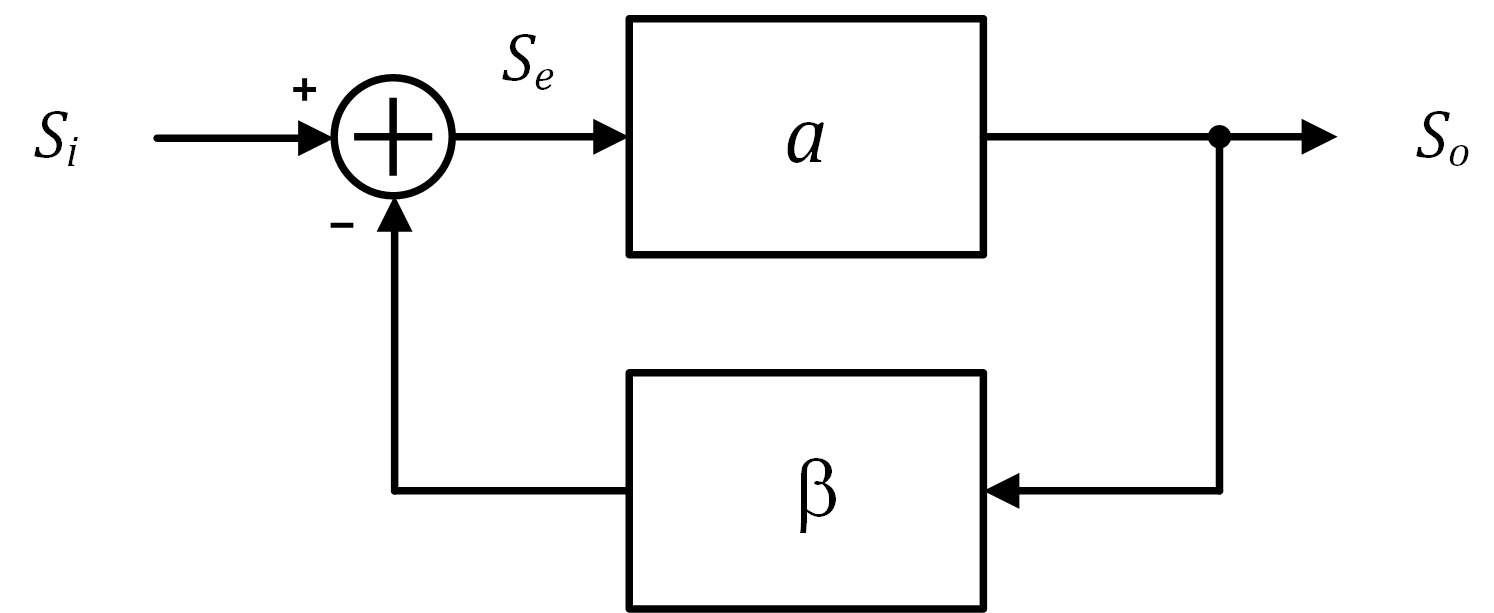
\includegraphics{negative_feedback.png}
\caption{negative\_feedback.png}
\end{figure}

    \begin{itemize}
\tightlist
\item
  Negative feedback loop processes the error
  \(S_i(s) -\beta \cdot S_o(s)\)
\item
  If the magnitude of \(a\) is large, the error is minimized,
  i.e.~\(S_i(s) - \beta \cdot S_o(s) \rightarrow 0\)
\item
  In this sense, negative feedback ``desensitizes'' the transfer
  function to the open-loop gain \(a\)
\end{itemize}

    \hypertarget{non-inverting-amplifier}{%
\subsection{Non-inverting amplifier}\label{non-inverting-amplifier}}

    \begin{figure}
\centering
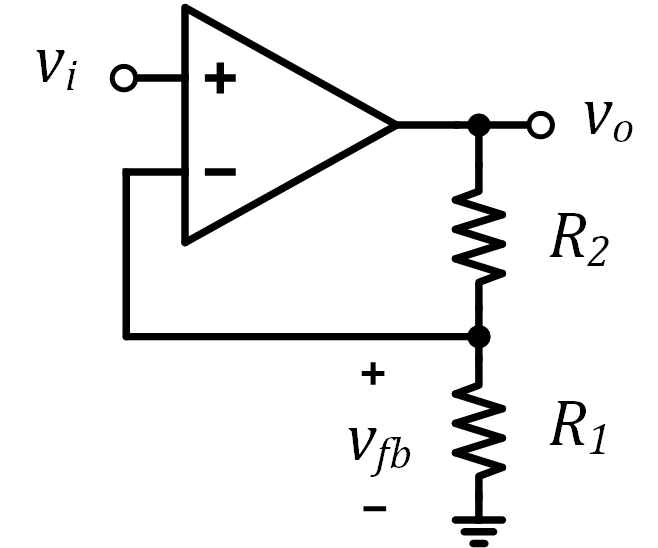
\includegraphics{non_inverting_amp.png}
\caption{non\_inverting\_amp.png}
\end{figure}

    \begin{equation}
a = A_{0}
\end{equation}

\begin{equation}
\beta = \dfrac{R_1}{R_1 + R_2}
\end{equation}

\begin{equation}
\dfrac{v_o}{v_i} = \dfrac{A_{0}}{1+\beta A_{0}} \approx \dfrac{1}{\beta}
\end{equation}

    \begin{itemize}
\tightlist
\item
  A fraction of the output voltage (set by \(\beta\)) is fed back to the
  inverting input and the error voltage is processed by the amplifier
\item
  Open-loop gain specification is determined by precision requirements
  (application-dependent)
\item
  Exact value of DC gain \(A_0\) is unimportant as long as it's ``large
  enough''
\end{itemize}

    \hypertarget{gain-bandwidth-product}{%
\subsection{Gain-bandwidth product}\label{gain-bandwidth-product}}

    \begin{figure}
\centering
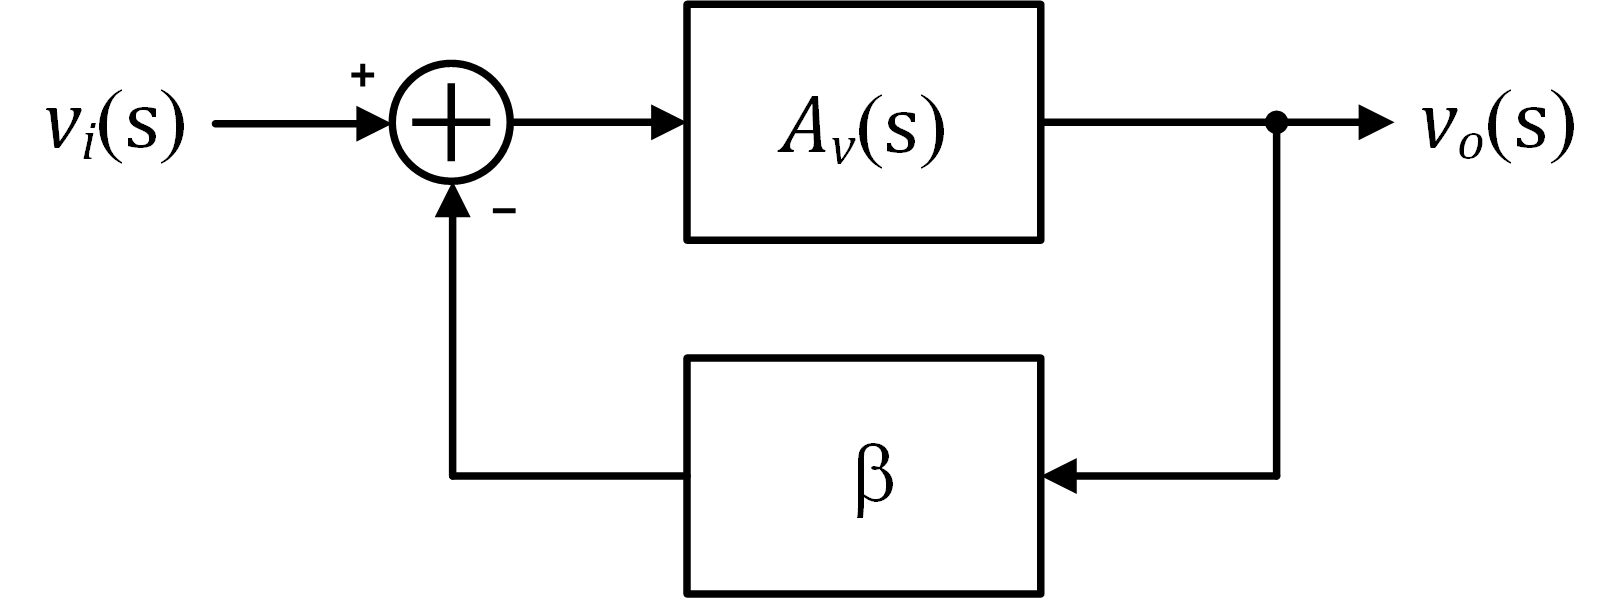
\includegraphics{feedback_frequency_response.png}
\caption{feedback\_frequency\_response.png}
\end{figure}

    \begin{equation}
G(s) = \dfrac{v_o(s)}{v_i(s)} = \dfrac{A_{v}(s)}{1+\beta A_{v}(s)}
\end{equation}

\begin{equation}
A_v(s) = \dfrac{A_0}{1+s/\omega_0}
\end{equation}

\begin{equation}
GBW = A_0 \omega_0
\end{equation}

    \begin{itemize}
\tightlist
\item
  Assuming dominant-pole behavior, we can readily assess the effect of
  negative feedback on frequency response
\item
  \(A_0\) is the \(DC\) gain of the \emph{open-loop} amplifier, and
  \(\omega_0\) is the dominant pole frequency (i.e.~\(3dB\) bandwidth)
\end{itemize}

    \begin{itemize}
\tightlist
\item
  To determine the frequency response of the closed-loop system, we
  substitute the frequency-dependent expression for \(A_v(s)\) into the
  closed-loop gain expression
\end{itemize}

\begin{equation}
G(s) = \dfrac{A_{v}(s)}{1+\beta A_{v}(s)} = \dfrac{A_0}{1+s/\omega_0 + \beta A_0} = \dfrac{\frac{A_0}{1+\beta A_0}}{1+\frac{s}{\omega_0 (1+\beta A_0)}}
\end{equation}

\begin{itemize}
\tightlist
\item
  Solving for the closed-loop pole frequency gives
\end{itemize}

\begin{equation}
\omega_0^{'} = \omega_0\cdot(1+\beta A_0)
\end{equation}

    \begin{tcolorbox}[breakable, size=fbox, boxrule=1pt, pad at break*=1mm,colback=cellbackground, colframe=cellborder]
\prompt{In}{incolor}{2}{\boxspacing}
\begin{Verbatim}[commandchars=\\\{\}]
\PY{k}{def} \PY{n+nf}{plot\PYZus{}CL\PYZus{}freq}\PY{p}{(}\PY{n}{A\PYZus{}dB}\PY{p}{,} \PY{n}{f\PYZus{}t}\PY{p}{,} \PY{n}{betas}\PY{p}{,} \PY{n}{w}\PY{p}{)}\PY{p}{:}
    \PY{n}{A\PYZus{}0} \PY{o}{=} \PY{l+m+mi}{10}\PY{o}{*}\PY{o}{*}\PY{p}{(}\PY{n}{A\PYZus{}dB}\PY{o}{/}\PY{l+m+mi}{20}\PY{p}{)}
    \PY{n}{f\PYZus{}3dB} \PY{o}{=} \PY{n}{f\PYZus{}t}\PY{o}{/}\PY{n}{A\PYZus{}0}
    \PY{n}{w\PYZus{}0} \PY{o}{=} \PY{n}{f\PYZus{}3dB}\PY{o}{*}\PY{l+m+mi}{2}\PY{o}{*}\PY{n}{np}\PY{o}{.}\PY{n}{pi}
    \PY{n}{A\PYZus{}s} \PY{o}{=} \PY{n}{np}\PY{o}{.}\PY{n}{array}\PY{p}{(}\PY{p}{[}\PY{p}{]}\PY{p}{)}

    \PY{n}{fig}\PY{p}{,} \PY{n}{axs} \PY{o}{=} \PY{n}{plt}\PY{o}{.}\PY{n}{subplots}\PY{p}{(}\PY{l+m+mi}{2}\PY{p}{,} \PY{n}{figsize}\PY{o}{=}\PY{p}{(}\PY{l+m+mf}{10.0}\PY{p}{,} \PY{l+m+mf}{8.0}\PY{p}{)}\PY{p}{)}
    \PY{k}{for} \PY{n}{b} \PY{o+ow}{in} \PY{n}{betas}\PY{p}{:}
        \PY{n}{Av\PYZus{}cl} \PY{o}{=} \PY{n}{signal}\PY{o}{.}\PY{n}{TransferFunction}\PY{p}{(}\PY{p}{[}\PY{n}{A\PYZus{}0}\PY{p}{]}\PY{p}{,} \PY{p}{[}\PY{l+m+mi}{1}\PY{o}{/}\PY{n}{w\PYZus{}0}\PY{p}{,} \PY{l+m+mi}{1} \PY{o}{+} \PY{n}{b}\PY{o}{*}\PY{n}{A\PYZus{}0}\PY{p}{]}\PY{p}{)}
        \PY{n}{w}\PY{p}{,} \PY{n}{mag}\PY{p}{,} \PY{n}{phase} \PY{o}{=} \PY{n}{Av\PYZus{}cl}\PY{o}{.}\PY{n}{bode}\PY{p}{(}\PY{n}{w}\PY{o}{=}\PY{n}{w}\PY{p}{)}       \PY{c+c1}{\PYZsh{} rad/s, dB, degrees }
        \PY{n}{f} \PY{o}{=} \PY{n}{w}\PY{o}{/}\PY{l+m+mi}{2}\PY{o}{/}\PY{n}{np}\PY{o}{.}\PY{n}{pi}   

        \PY{c+c1}{\PYZsh{} Plot the frequency response for multiple values of beta}
        \PY{n}{fig}\PY{o}{.}\PY{n}{suptitle}\PY{p}{(}\PY{l+s+s1}{\PYZsq{}}\PY{l+s+s1}{Opamp Closed\PYZhy{}Loop Frequency Response}\PY{l+s+s1}{\PYZsq{}}\PY{p}{)}
        \PY{n}{axs}\PY{p}{[}\PY{l+m+mi}{0}\PY{p}{]}\PY{o}{.}\PY{n}{semilogx}\PY{p}{(}\PY{n}{f}\PY{p}{,} \PY{n}{mag}\PY{p}{)}
        \PY{n}{axs}\PY{p}{[}\PY{l+m+mi}{0}\PY{p}{]}\PY{o}{.}\PY{n}{grid}\PY{p}{(}\PY{p}{)}
        \PY{n}{axs}\PY{p}{[}\PY{l+m+mi}{0}\PY{p}{]}\PY{o}{.}\PY{n}{set\PYZus{}ylabel}\PY{p}{(}\PY{l+s+s1}{\PYZsq{}}\PY{l+s+s1}{Magnitude [dB]}\PY{l+s+s1}{\PYZsq{}}\PY{p}{)}
        \PY{n}{axs}\PY{p}{[}\PY{l+m+mi}{1}\PY{p}{]}\PY{o}{.}\PY{n}{semilogx}\PY{p}{(}\PY{n}{f}\PY{p}{,}\PY{n}{phase}\PY{p}{)}
        \PY{n}{axs}\PY{p}{[}\PY{l+m+mi}{1}\PY{p}{]}\PY{o}{.}\PY{n}{grid}\PY{p}{(}\PY{p}{)}
        \PY{n}{axs}\PY{p}{[}\PY{l+m+mi}{1}\PY{p}{]}\PY{o}{.}\PY{n}{set\PYZus{}ylabel}\PY{p}{(}\PY{l+s+s1}{\PYZsq{}}\PY{l+s+s1}{Phase [deg]}\PY{l+s+s1}{\PYZsq{}}\PY{p}{)}
        \PY{n}{axs}\PY{p}{[}\PY{l+m+mi}{1}\PY{p}{]}\PY{o}{.}\PY{n}{set\PYZus{}xlabel}\PY{p}{(}\PY{l+s+s1}{\PYZsq{}}\PY{l+s+s1}{Frequency [Hz]}\PY{l+s+s1}{\PYZsq{}}\PY{p}{)}
        \PY{n}{fig}\PY{o}{.}\PY{n}{align\PYZus{}ylabels}\PY{p}{(}\PY{n}{axs}\PY{p}{[}\PY{p}{:}\PY{p}{]}\PY{p}{)}
        
\PY{k}{def} \PY{n+nf}{plot\PYZus{}CL\PYZus{}step}\PY{p}{(}\PY{n}{A\PYZus{}dB}\PY{p}{,} \PY{n}{f\PYZus{}t}\PY{p}{,} \PY{n}{betas}\PY{p}{,} \PY{n}{w}\PY{p}{)}\PY{p}{:}
    \PY{n}{A\PYZus{}0} \PY{o}{=} \PY{l+m+mi}{10}\PY{o}{*}\PY{o}{*}\PY{p}{(}\PY{n}{A\PYZus{}dB}\PY{o}{/}\PY{l+m+mi}{20}\PY{p}{)}
    \PY{n}{f\PYZus{}3dB} \PY{o}{=} \PY{n}{f\PYZus{}t}\PY{o}{/}\PY{n}{A\PYZus{}0}
    \PY{n}{w\PYZus{}0} \PY{o}{=} \PY{n}{f\PYZus{}3dB}\PY{o}{*}\PY{l+m+mi}{2}\PY{o}{*}\PY{n}{np}\PY{o}{.}\PY{n}{pi}
    \PY{n}{A\PYZus{}s} \PY{o}{=} \PY{n}{np}\PY{o}{.}\PY{n}{array}\PY{p}{(}\PY{p}{[}\PY{p}{]}\PY{p}{)}
    
    \PY{n}{fig}\PY{p}{,} \PY{n}{axs} \PY{o}{=} \PY{n}{plt}\PY{o}{.}\PY{n}{subplots}\PY{p}{(}\PY{l+m+mi}{2}\PY{p}{,} \PY{n}{figsize}\PY{o}{=}\PY{p}{(}\PY{l+m+mf}{10.0}\PY{p}{,} \PY{l+m+mf}{8.0}\PY{p}{)}\PY{p}{)}
    \PY{k}{for} \PY{n}{b} \PY{o+ow}{in} \PY{n}{betas}\PY{p}{:}
        \PY{n}{Av\PYZus{}cl} \PY{o}{=} \PY{n}{signal}\PY{o}{.}\PY{n}{TransferFunction}\PY{p}{(}\PY{p}{[}\PY{n}{A\PYZus{}0}\PY{p}{]}\PY{p}{,} \PY{p}{[}\PY{l+m+mi}{1}\PY{o}{/}\PY{n}{w\PYZus{}0}\PY{p}{,} \PY{l+m+mi}{1} \PY{o}{+} \PY{n}{b}\PY{o}{*}\PY{n}{A\PYZus{}0}\PY{p}{]}\PY{p}{)}
        \PY{n}{tin} \PY{o}{=} \PY{n}{np}\PY{o}{.}\PY{n}{linspace}\PY{p}{(}\PY{l+m+mi}{0}\PY{p}{,}\PY{l+m+mf}{20e\PYZhy{}6}\PY{p}{,}\PY{l+m+mi}{100}\PY{p}{)}
        \PY{n}{u\PYZus{}step} \PY{o}{=} \PY{n}{np}\PY{o}{.}\PY{n}{concatenate}\PY{p}{(} \PY{p}{(}\PY{l+m+mi}{0}\PY{p}{,} \PY{n}{np}\PY{o}{.}\PY{n}{ones}\PY{p}{(}\PY{l+m+mi}{99}\PY{p}{)}\PY{p}{)}\PY{p}{,} \PY{n}{axis}\PY{o}{=}\PY{k+kc}{None}\PY{p}{)}
        \PY{n}{tout}\PY{p}{,}\PY{n}{vout} \PY{o}{=} \PY{n}{signal}\PY{o}{.}\PY{n}{step}\PY{p}{(}\PY{n}{Av\PYZus{}cl}\PY{p}{,} \PY{n}{X0}\PY{o}{=}\PY{k+kc}{None}\PY{p}{,} \PY{n}{T}\PY{o}{=}\PY{n}{tin}\PY{p}{)}

        \PY{c+c1}{\PYZsh{} Plot the step response for multiple values of beta}
        \PY{n}{fig}\PY{o}{.}\PY{n}{suptitle}\PY{p}{(}\PY{l+s+s1}{\PYZsq{}}\PY{l+s+s1}{Opamp Closed\PYZhy{}Loop Step Response}\PY{l+s+s1}{\PYZsq{}}\PY{p}{)}
        \PY{n}{axs}\PY{p}{[}\PY{l+m+mi}{0}\PY{p}{]}\PY{o}{.}\PY{n}{plot}\PY{p}{(}\PY{l+m+mf}{1e6}\PY{o}{*}\PY{n}{tout}\PY{p}{,} \PY{n}{b}\PY{o}{*}\PY{n}{vout}\PY{p}{)}
        \PY{n}{axs}\PY{p}{[}\PY{l+m+mi}{0}\PY{p}{]}\PY{o}{.}\PY{n}{grid}\PY{p}{(}\PY{p}{)}
        \PY{n}{axs}\PY{p}{[}\PY{l+m+mi}{0}\PY{p}{]}\PY{o}{.}\PY{n}{set\PYZus{}ylabel}\PY{p}{(}\PY{l+s+sa}{r}\PY{l+s+s1}{\PYZsq{}}\PY{l+s+s1}{\PYZdl{}}\PY{l+s+s1}{\PYZbs{}}\PY{l+s+s1}{beta V\PYZus{}o\PYZdl{} [V]}\PY{l+s+s1}{\PYZsq{}}\PY{p}{)}
        \PY{n}{axs}\PY{p}{[}\PY{l+m+mi}{1}\PY{p}{]}\PY{o}{.}\PY{n}{plot}\PY{p}{(}\PY{l+m+mf}{1e6}\PY{o}{*}\PY{n}{tin}\PY{p}{,}\PY{n}{u\PYZus{}step}\PY{p}{)}
        \PY{n}{axs}\PY{p}{[}\PY{l+m+mi}{1}\PY{p}{]}\PY{o}{.}\PY{n}{grid}\PY{p}{(}\PY{p}{)}
        \PY{n}{axs}\PY{p}{[}\PY{l+m+mi}{1}\PY{p}{]}\PY{o}{.}\PY{n}{set\PYZus{}ylabel}\PY{p}{(}\PY{l+s+s1}{\PYZsq{}}\PY{l+s+s1}{Input Voltage [V]}\PY{l+s+s1}{\PYZsq{}}\PY{p}{)}
        \PY{n}{axs}\PY{p}{[}\PY{l+m+mi}{1}\PY{p}{]}\PY{o}{.}\PY{n}{set\PYZus{}xlabel}\PY{p}{(}\PY{l+s+s1}{\PYZsq{}}\PY{l+s+s1}{Time [\PYZdl{}}\PY{l+s+s1}{\PYZbs{}}\PY{l+s+s1}{mu \PYZdl{}s]}\PY{l+s+s1}{\PYZsq{}}\PY{p}{)}
        \PY{n}{fig}\PY{o}{.}\PY{n}{align\PYZus{}ylabels}\PY{p}{(}\PY{n}{axs}\PY{p}{[}\PY{p}{:}\PY{p}{]}\PY{p}{)}
\end{Verbatim}
\end{tcolorbox}

    \hypertarget{gain-bandwidth-bode}{%
\subsection{Gain-bandwidth (Bode)}\label{gain-bandwidth-bode}}

    \begin{figure}
\centering
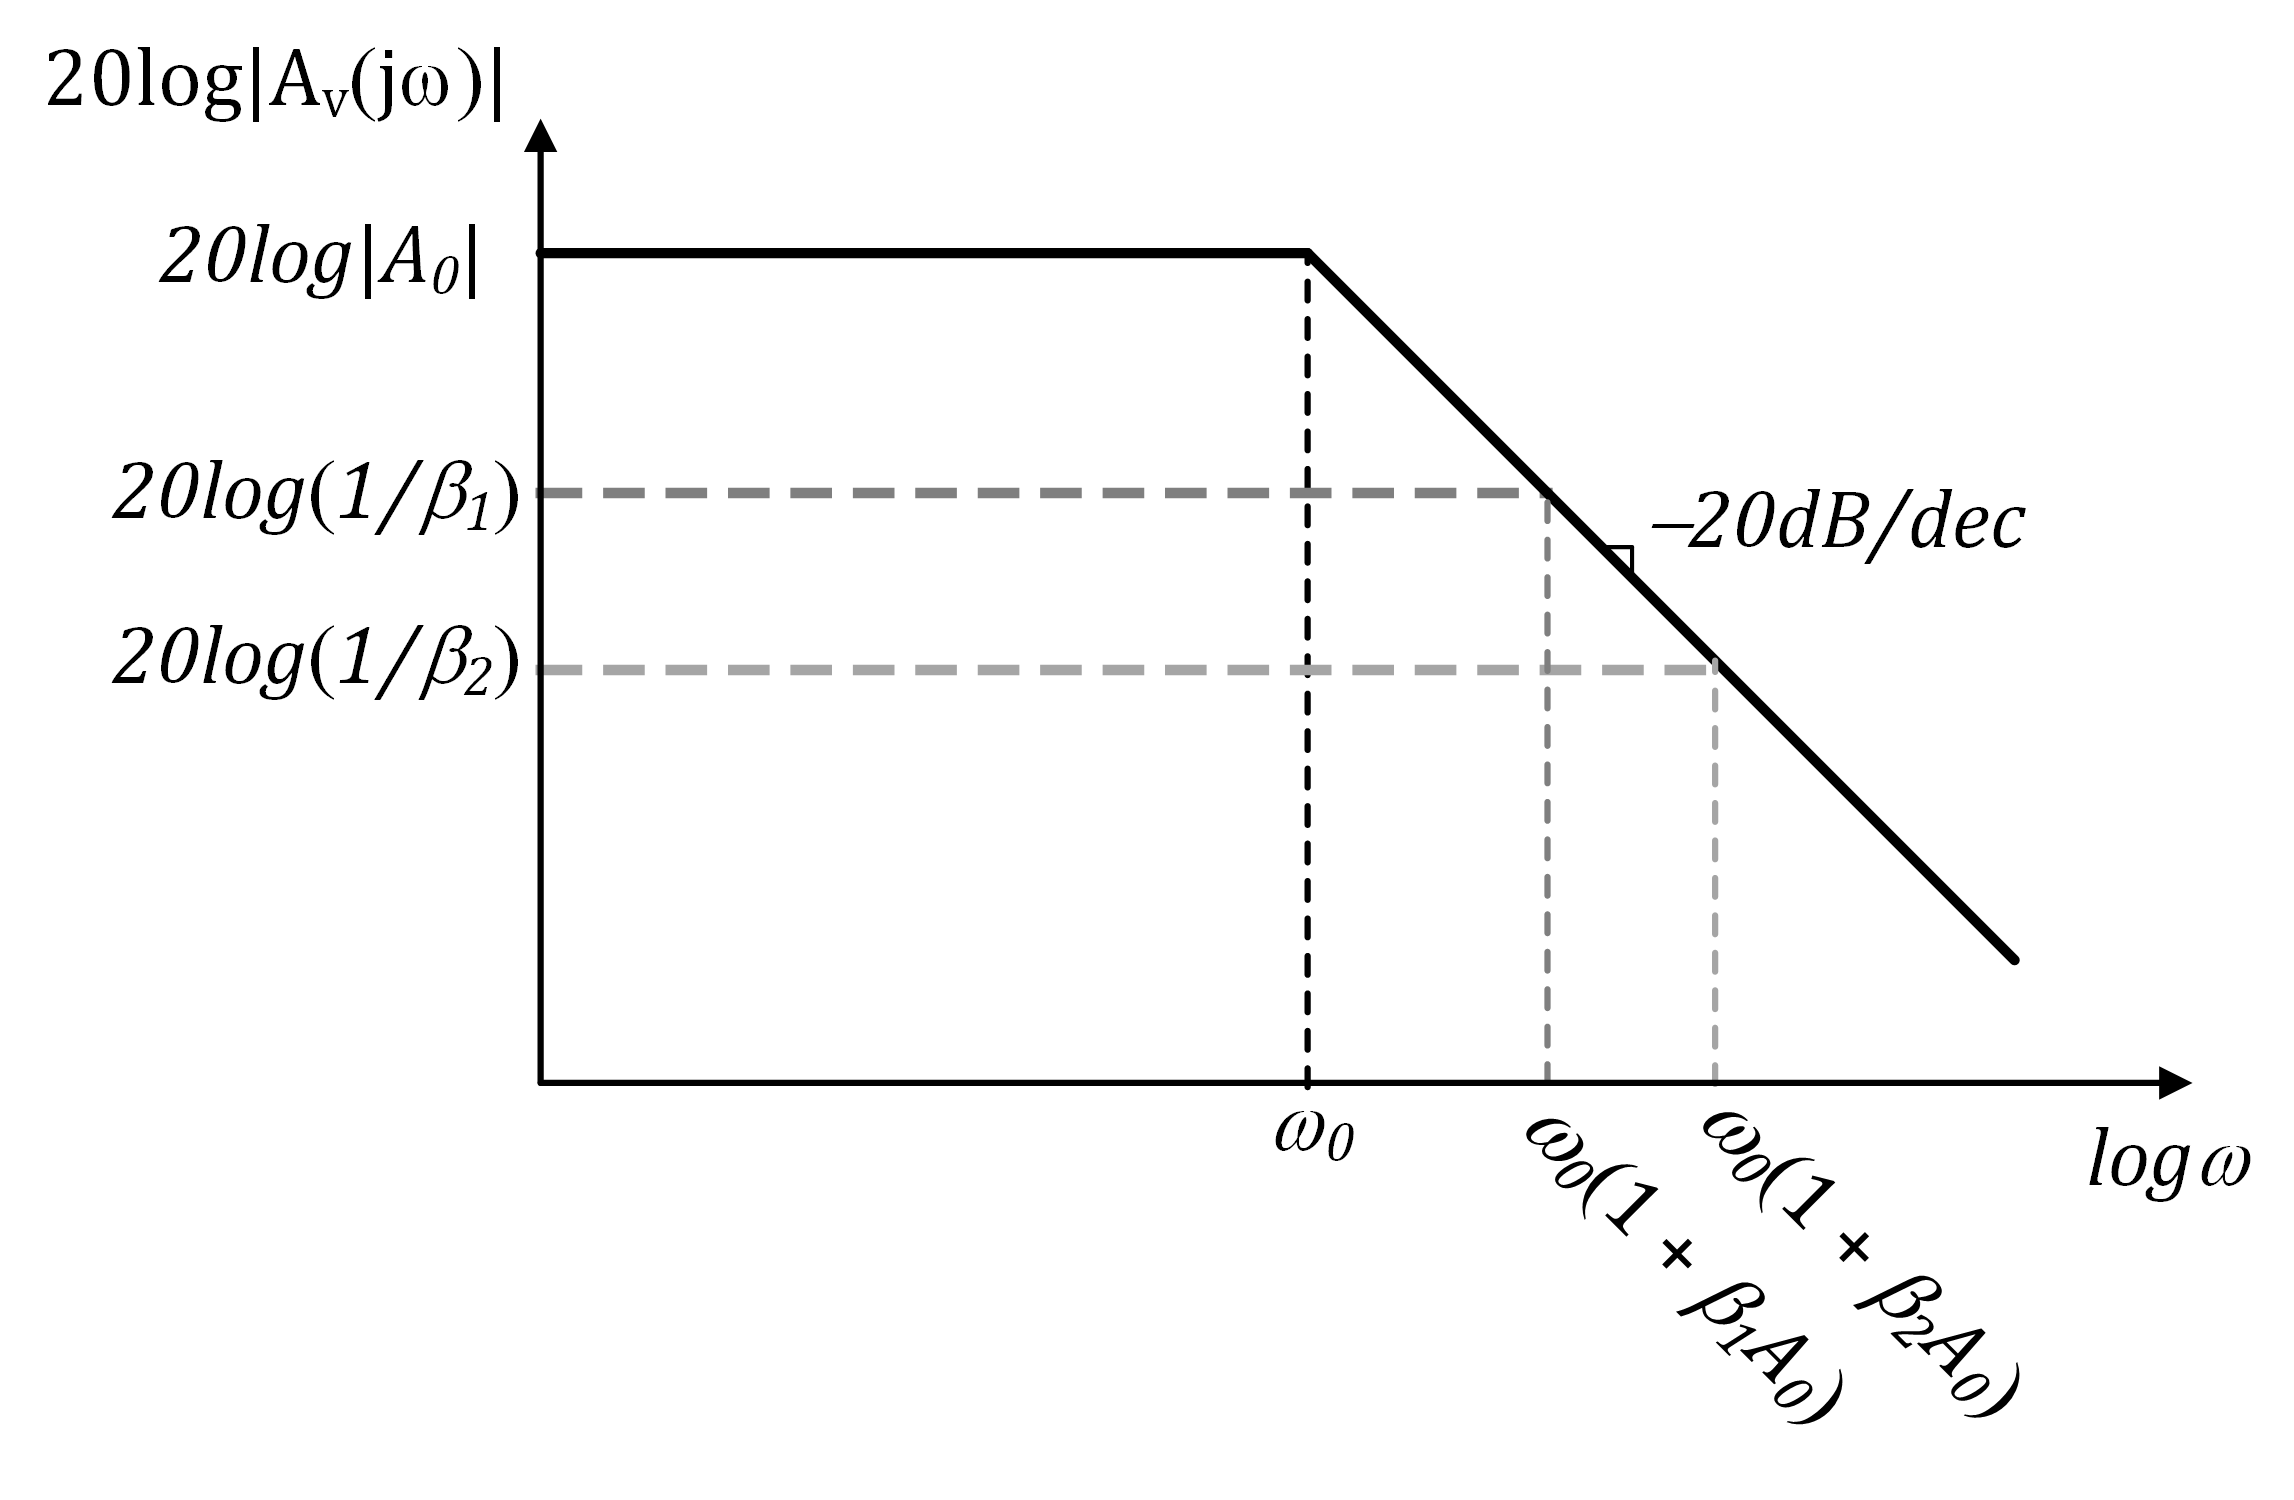
\includegraphics{closed_loop_bode.png}
\caption{closed\_loop\_bode.png}
\end{figure}

    \begin{equation}
A_v(s) = \dfrac{A_0}{1+s/\omega_0}
\end{equation}

\begin{equation}
G(s) = \dfrac{\frac{A_0}{1+\beta A_0}}{1+\frac{s}{\omega_0 (1+\beta A_0)}}
\end{equation}

\begin{equation}
\omega_0^{'} = \omega_0\cdot(1+\beta A_0)
\end{equation}

    \begin{itemize}
\tightlist
\item
  For every \(20dB\) reduction in closed-loop gain, the \(3dB\)
  frequency increases by 1 decade
\item
  This results from a constant gain-bandwidth product, which is an
  intrinsic property of the open-loop amplifier
\item
  Note that this assumes that the impedances in the feedback network are
  purely real (i.e.~resistors only)
\end{itemize}

    \begin{itemize}
\tightlist
\item
  Let's take a look at the closed-loop frequency response as a function
  of the feedback factor \(\beta\)
\end{itemize}

    \begin{tcolorbox}[breakable, size=fbox, boxrule=1pt, pad at break*=1mm,colback=cellbackground, colframe=cellborder]
\prompt{In}{incolor}{3}{\boxspacing}
\begin{Verbatim}[commandchars=\\\{\}]
\PY{n}{betas} \PY{o}{=} \PY{n}{np}\PY{o}{.}\PY{n}{logspace}\PY{p}{(}\PY{o}{\PYZhy{}}\PY{l+m+mi}{4}\PY{p}{,} \PY{l+m+mi}{0}\PY{p}{,} \PY{n}{num}\PY{o}{=}\PY{l+m+mi}{5}\PY{p}{)}
\PY{n}{w} \PY{o}{=} \PY{l+m+mi}{2}\PY{o}{*}\PY{n}{np}\PY{o}{.}\PY{n}{pi}\PY{o}{*}\PY{n}{np}\PY{o}{.}\PY{n}{logspace}\PY{p}{(}\PY{l+m+mi}{0}\PY{p}{,}\PY{l+m+mi}{9}\PY{p}{,}\PY{n}{num}\PY{o}{=}\PY{l+m+mi}{100}\PY{p}{)}
\PY{n}{plot\PYZus{}CL\PYZus{}freq}\PY{p}{(}\PY{l+m+mi}{120}\PY{p}{,} \PY{l+m+mf}{10e6}\PY{p}{,} \PY{n}{betas}\PY{p}{,} \PY{n}{w}\PY{p}{)}
\end{Verbatim}
\end{tcolorbox}

    \begin{center}
    \adjustimage{max size={0.9\linewidth}{0.9\paperheight}}{2021_02_24_EE538_Lecture8_W2021_files/2021_02_24_EE538_Lecture8_W2021_28_0.png}
    \end{center}
    { \hspace*{\fill} \\}
    
    \hypertarget{stability-barkhausen-criteria}{%
\subsection{Stability: Barkhausen
criteria}\label{stability-barkhausen-criteria}}

    \begin{figure}
\centering
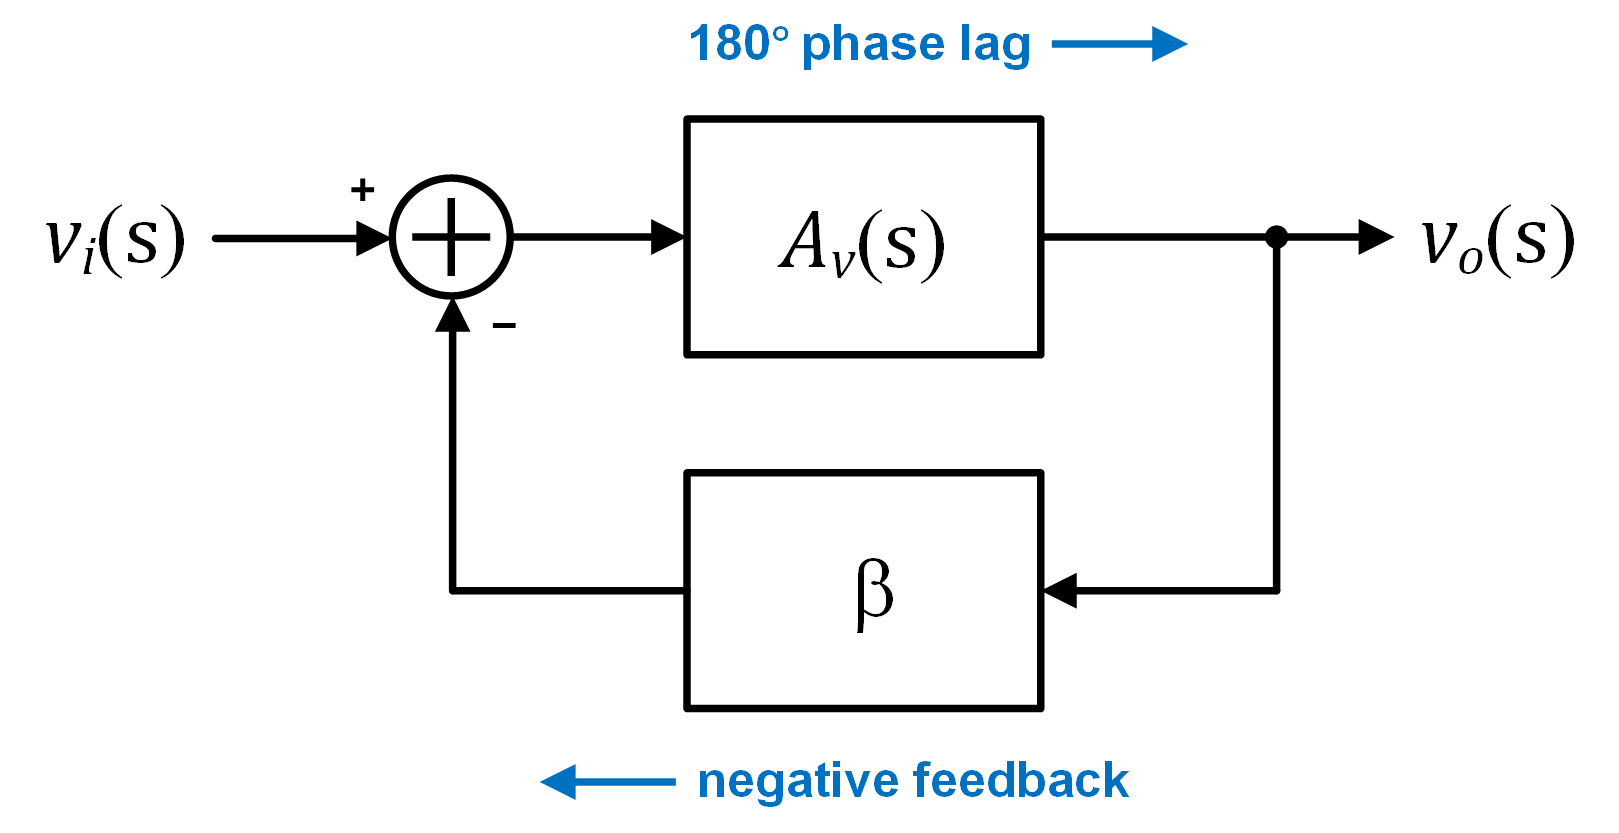
\includegraphics{barkhausen_criteria.png}
\caption{barkhausen\_criteria.png}
\end{figure}

    \begin{itemize}
\tightlist
\item
  In a negative feedback loop, if the loop gain at a given frequency
  \(\omega_1\) is \(-1\), the circuit may oscillate
\item
  This corresponds to a loop gain magnitude
  \(|\beta A_v(j\omega_1)| = 1\) and phase
  \(\angle A_v(j\omega_1) = -180^{\circ}\)
\end{itemize}

    \hypertarget{stability-root-locus}{%
\subsection{Stability: Root locus}\label{stability-root-locus}}

    \begin{itemize}
\tightlist
\item
  Open-loop transfer function
\end{itemize}

\begin{equation}
A_v(s) = \dfrac{A_0}{1+\dfrac{s}{\omega_0}}
\end{equation}

\begin{itemize}
\tightlist
\item
  Closed-loop transfer function
\end{itemize}

\begin{equation}
G(s) = \dfrac{A_0}{1+s/\omega_0 + \beta A_0}
\end{equation}

    \begin{itemize}
\tightlist
\item
  Open-loop pole
\end{itemize}

\begin{equation}
s_0 = -\omega_0
\end{equation}

\begin{itemize}
\tightlist
\item
  Closed-loop pole
\end{itemize}

\begin{equation}
s_0^{'} = -\omega_0(1+\beta A_0)
\end{equation}

    \begin{itemize}
\item
  Root locus plots involve plotting the closed-loop poles in the complex
  plane to evaluate stability
\item
  If a given pole \(s = j\omega + \sigma\) falls in the right half plane
  (\(RHP\)), the system is unstable (phase lag \(> 180^{\circ}\))
\item
  Here, for a single pole system, we have a single, real, \(LHP\) pole,
  so the system is unconditionally stable
\end{itemize}

    \hypertarget{bode-plot-vs-root-locus}{%
\subsection{Bode plot vs root locus}\label{bode-plot-vs-root-locus}}

    \begin{figure}
\centering
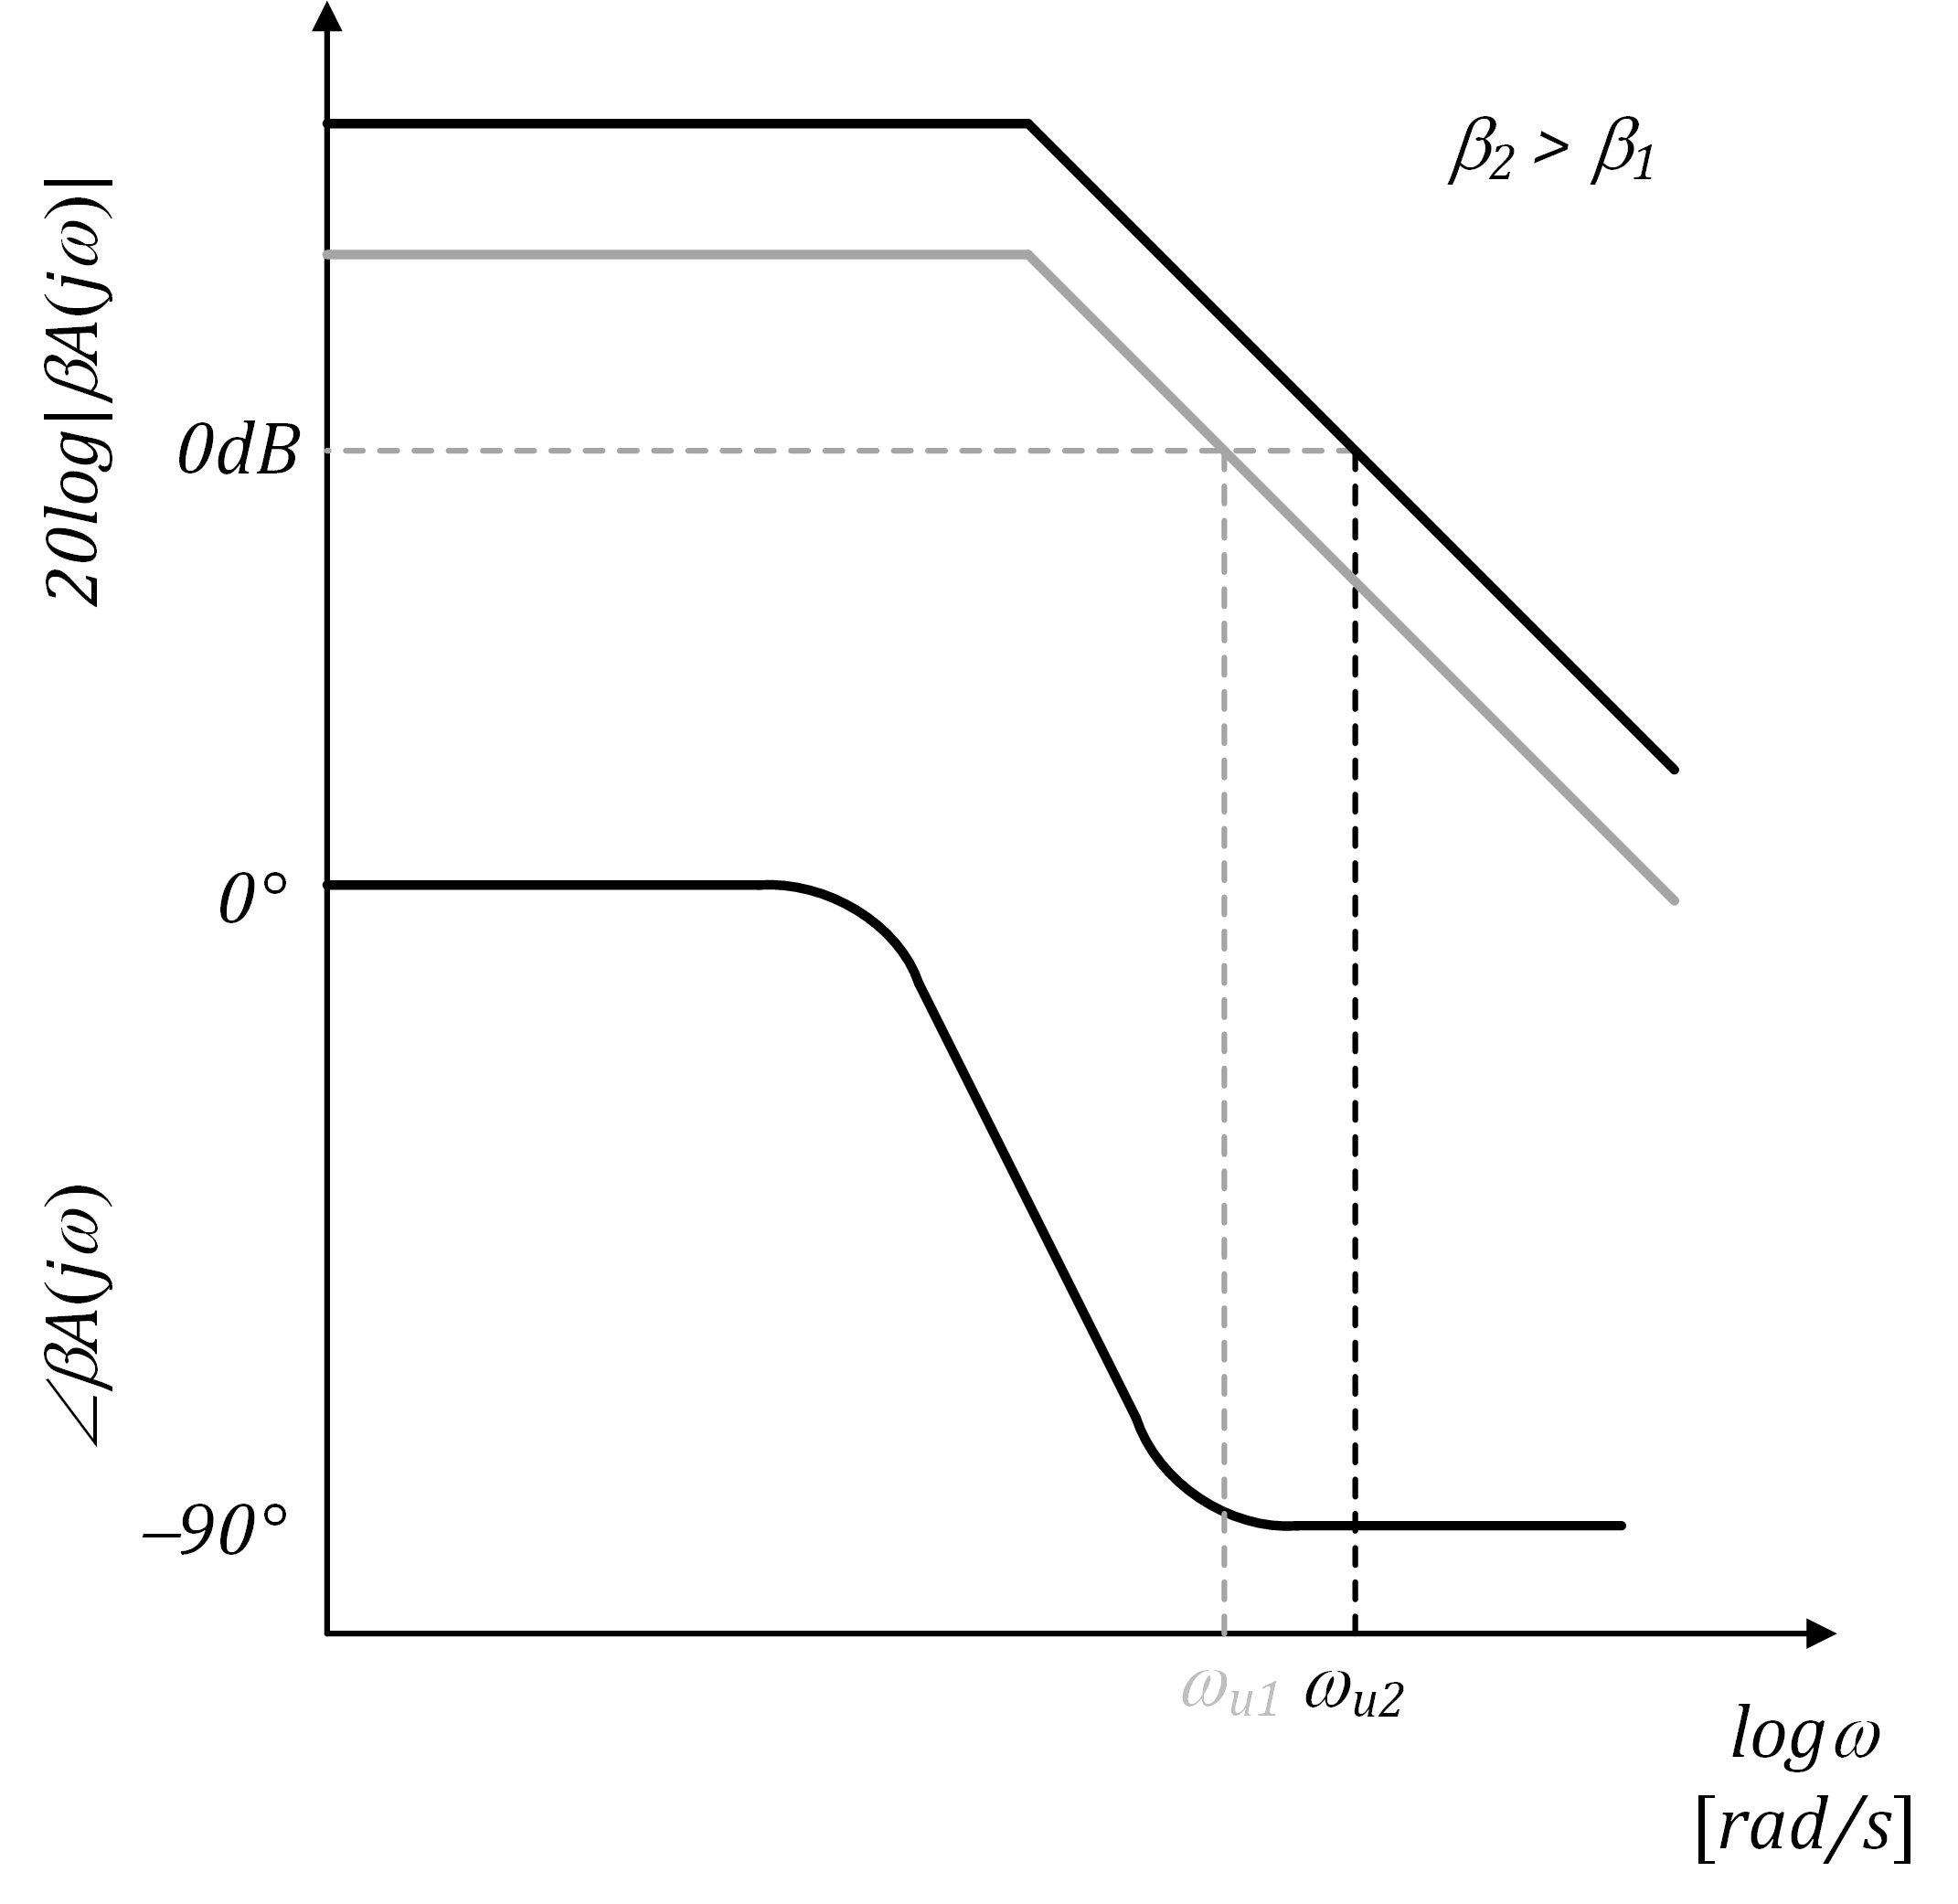
\includegraphics{bode_plot.png}
\caption{bode\_plot.png}
\end{figure}

    \begin{figure}
\centering
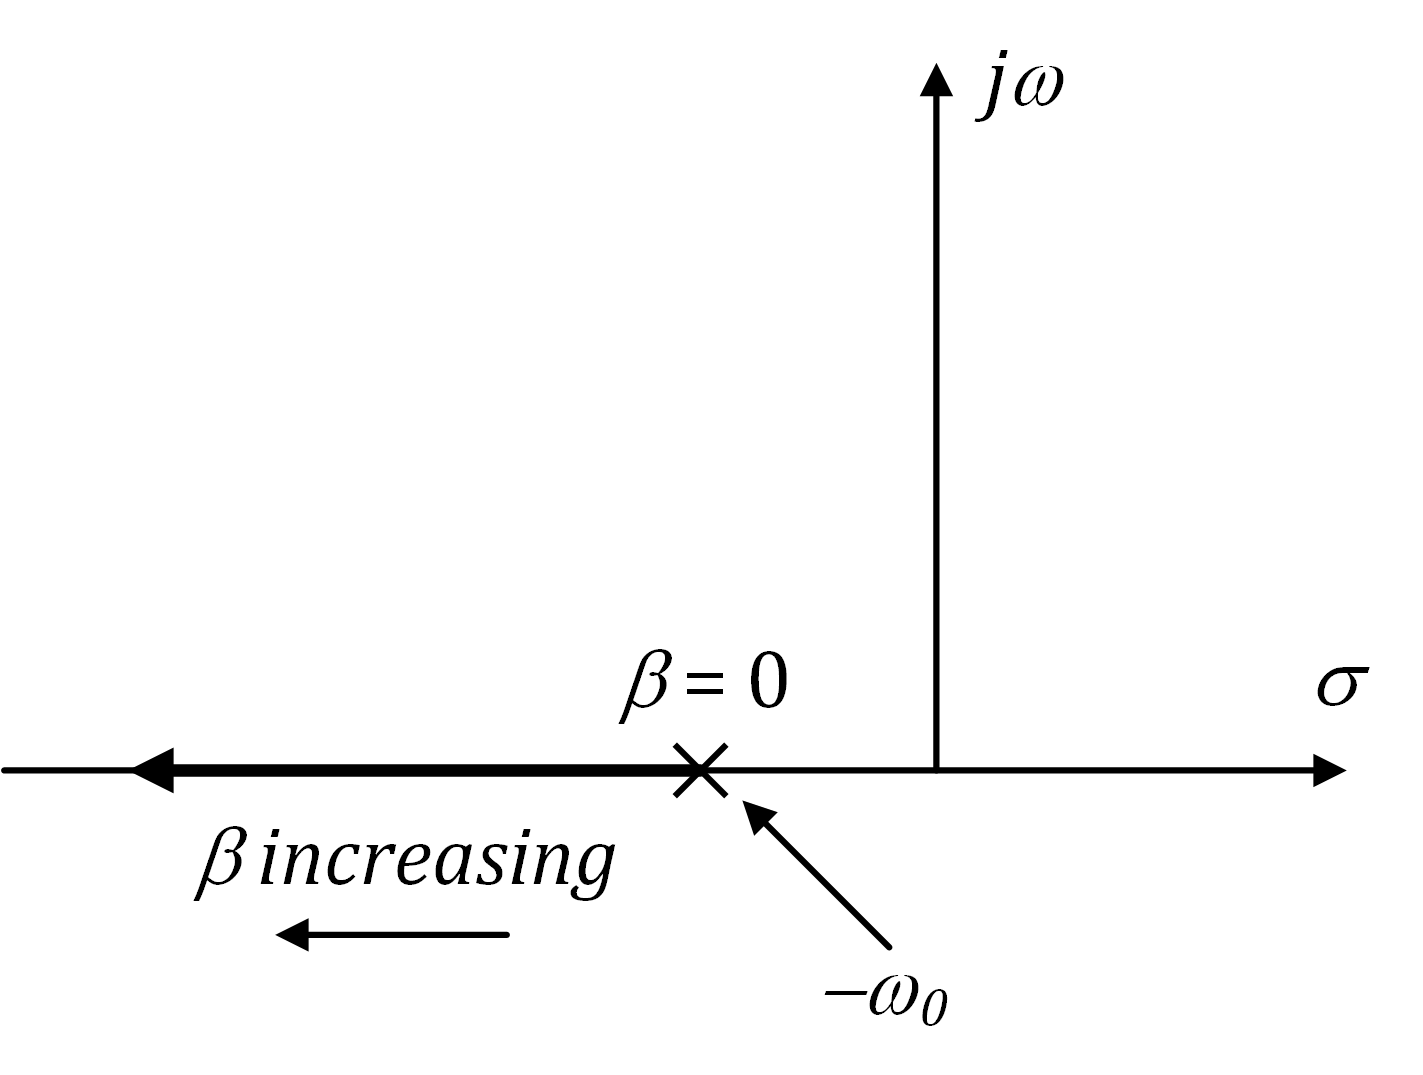
\includegraphics{root_locus_first_order.png}
\caption{root\_locus\_first\_order.png}
\end{figure}

    \begin{itemize}
\tightlist
\item
  For a single-pole system both methods indicate unconditional
  stability:

  \begin{itemize}
  \tightlist
  \item
    Bode plot: Maximum phase lag of \(90^{\circ}\)
  \item
    Root locus: Purely real, \(LHP\) pole
  \end{itemize}
\item
  For higher-order systems, the worst-case scenario arises when
  \(\beta = 1\) (highest possible loop gain)
\end{itemize}

    \hypertarget{root-locus-of-a-second-order-system}{%
\subsection{Root locus of a second-order
system}\label{root-locus-of-a-second-order-system}}

    \begin{itemize}
\tightlist
\item
  Open-loop transfer function
\end{itemize}

\begin{equation}
A_v(s) = \dfrac{A_0}{\left(1+\dfrac{s}{\omega_{p1}} \right) \left(1+\dfrac{s}{\omega_{p2}} \right)}
\end{equation}

\begin{itemize}
\tightlist
\item
  Closed-loop transfer function
\end{itemize}

\begin{equation}
A_v(s) = \dfrac{A_0}{\left(1+\dfrac{s}{\omega_{p1}} \right) \left(1+\dfrac{s}{\omega_{p2}} \right) + \beta A_0}
\end{equation}

    \begin{itemize}
\item
  For a second-order system, the situation is more ``complex''
\item
  We can solve for the closed-loop pole locations using the quadratic
  formula and plot them in the complex plane to evaluate stability
\end{itemize}

    \begin{figure}
\centering
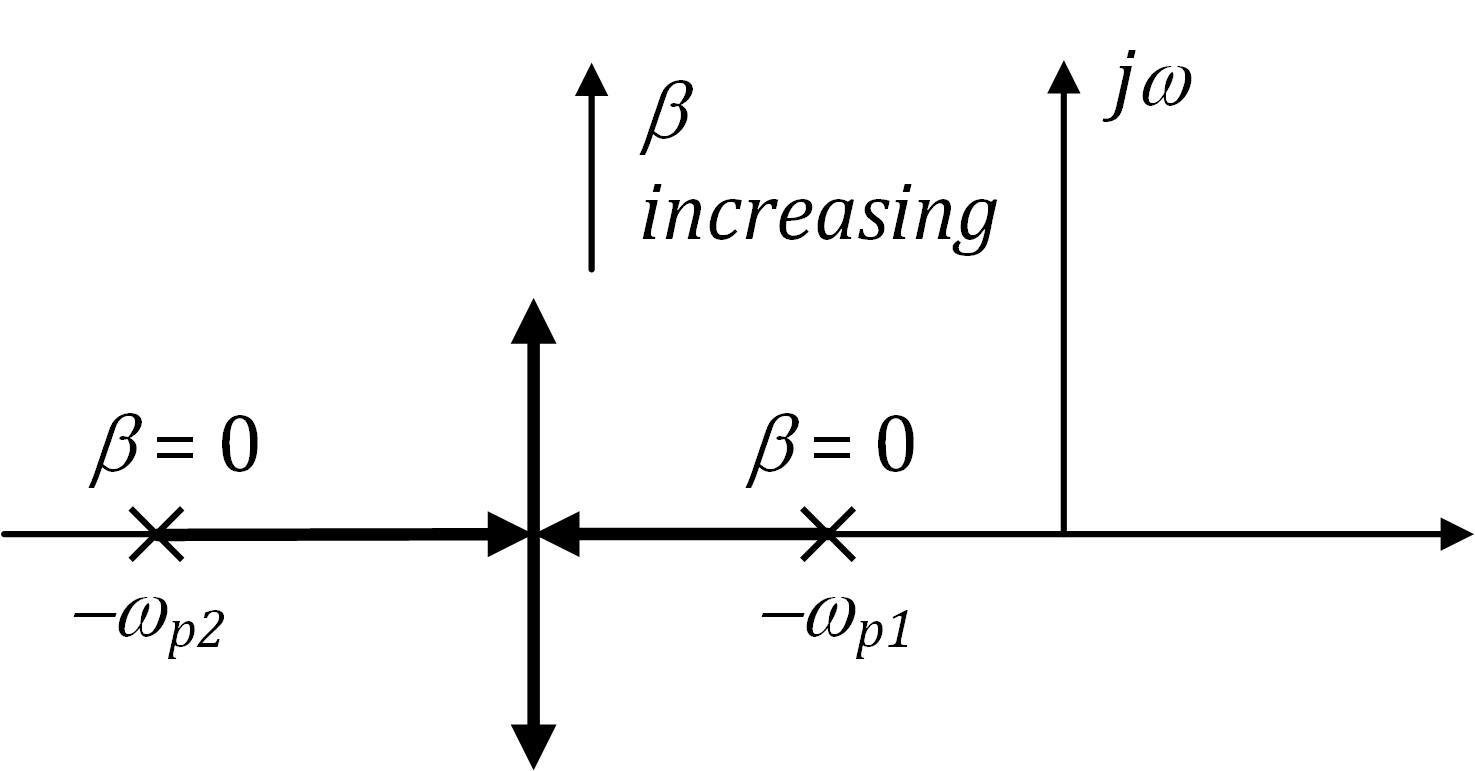
\includegraphics{root_locus_second_order.png}
\caption{root\_locus\_second\_order.png}
\end{figure}

    \begin{itemize}
\tightlist
\item
  The closed-loop poles are given by
\end{itemize}

\begin{equation}
s_{p1,2} = \dfrac{-(\omega_{p1} + \omega_{p2})\pm \sqrt{(\omega_{p1}+\omega_{p2})^2 - 4(1+\beta A_0)\omega_{p1} \omega_{p2}}}{2}
\end{equation}

\begin{itemize}
\tightlist
\item
  When \(\beta = 0\) (no feedback), the closed-loop poles are equal to
  the open-loop poles
\item
  As \(\beta\) increases, the imaginary components of \(s_{p1}\) and
  \(s_{p2}\) increase
\end{itemize}

    \hypertarget{damping-ratio-and-phase-margin}{%
\subsection{Damping ratio and phase
margin}\label{damping-ratio-and-phase-margin}}

    \begin{figure}
\centering
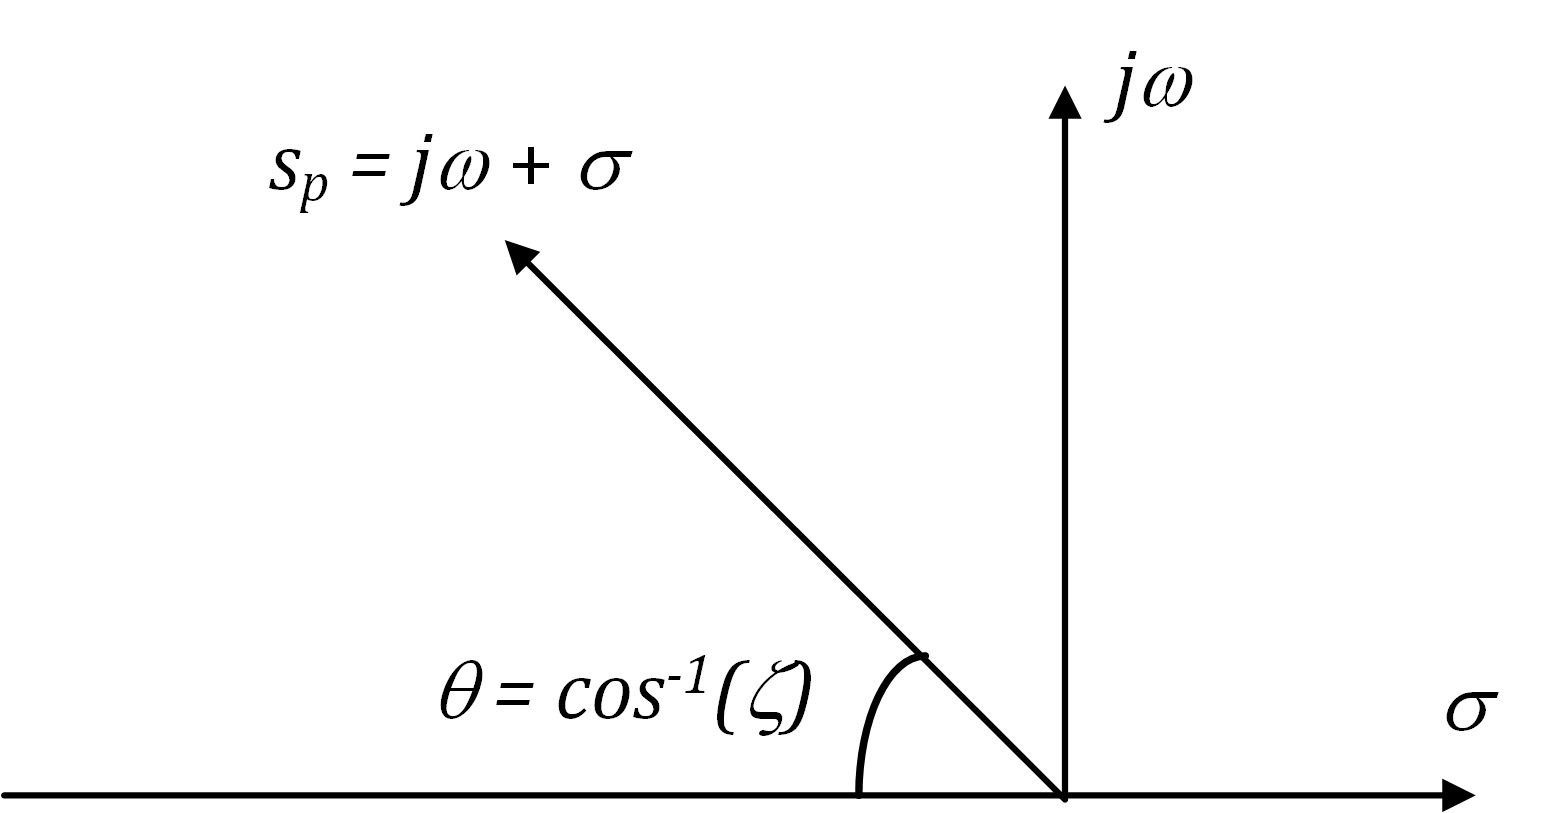
\includegraphics{damping_ratio.png}
\caption{damping\_ratio.png}
\end{figure}

    \begin{equation}
PM = \tan^{-1}\dfrac{2\zeta}{-2\zeta^2 + \sqrt{1+4\zeta^2}}
\end{equation}

    \begin{itemize}
\item
  As \(\beta\) increases, the angle \(\cos^{-1}(\zeta)\) increases, the
  magnitude of the imaginary component increases relative to that of the
  real component
\item
  \(\zeta\) is referred to as the ``damping factor,'' and can be used to
  evaluate the qualitative behavior of the impulse response
\item
  Another means of evaluating this behavior is by looking at the phase
  margin, which enables use of the Bode plot
\end{itemize}

    \hypertarget{phase-margin-of-a-single-pole-system}{%
\subsection{Phase margin of a single-pole
system}\label{phase-margin-of-a-single-pole-system}}

    \begin{figure}
\centering
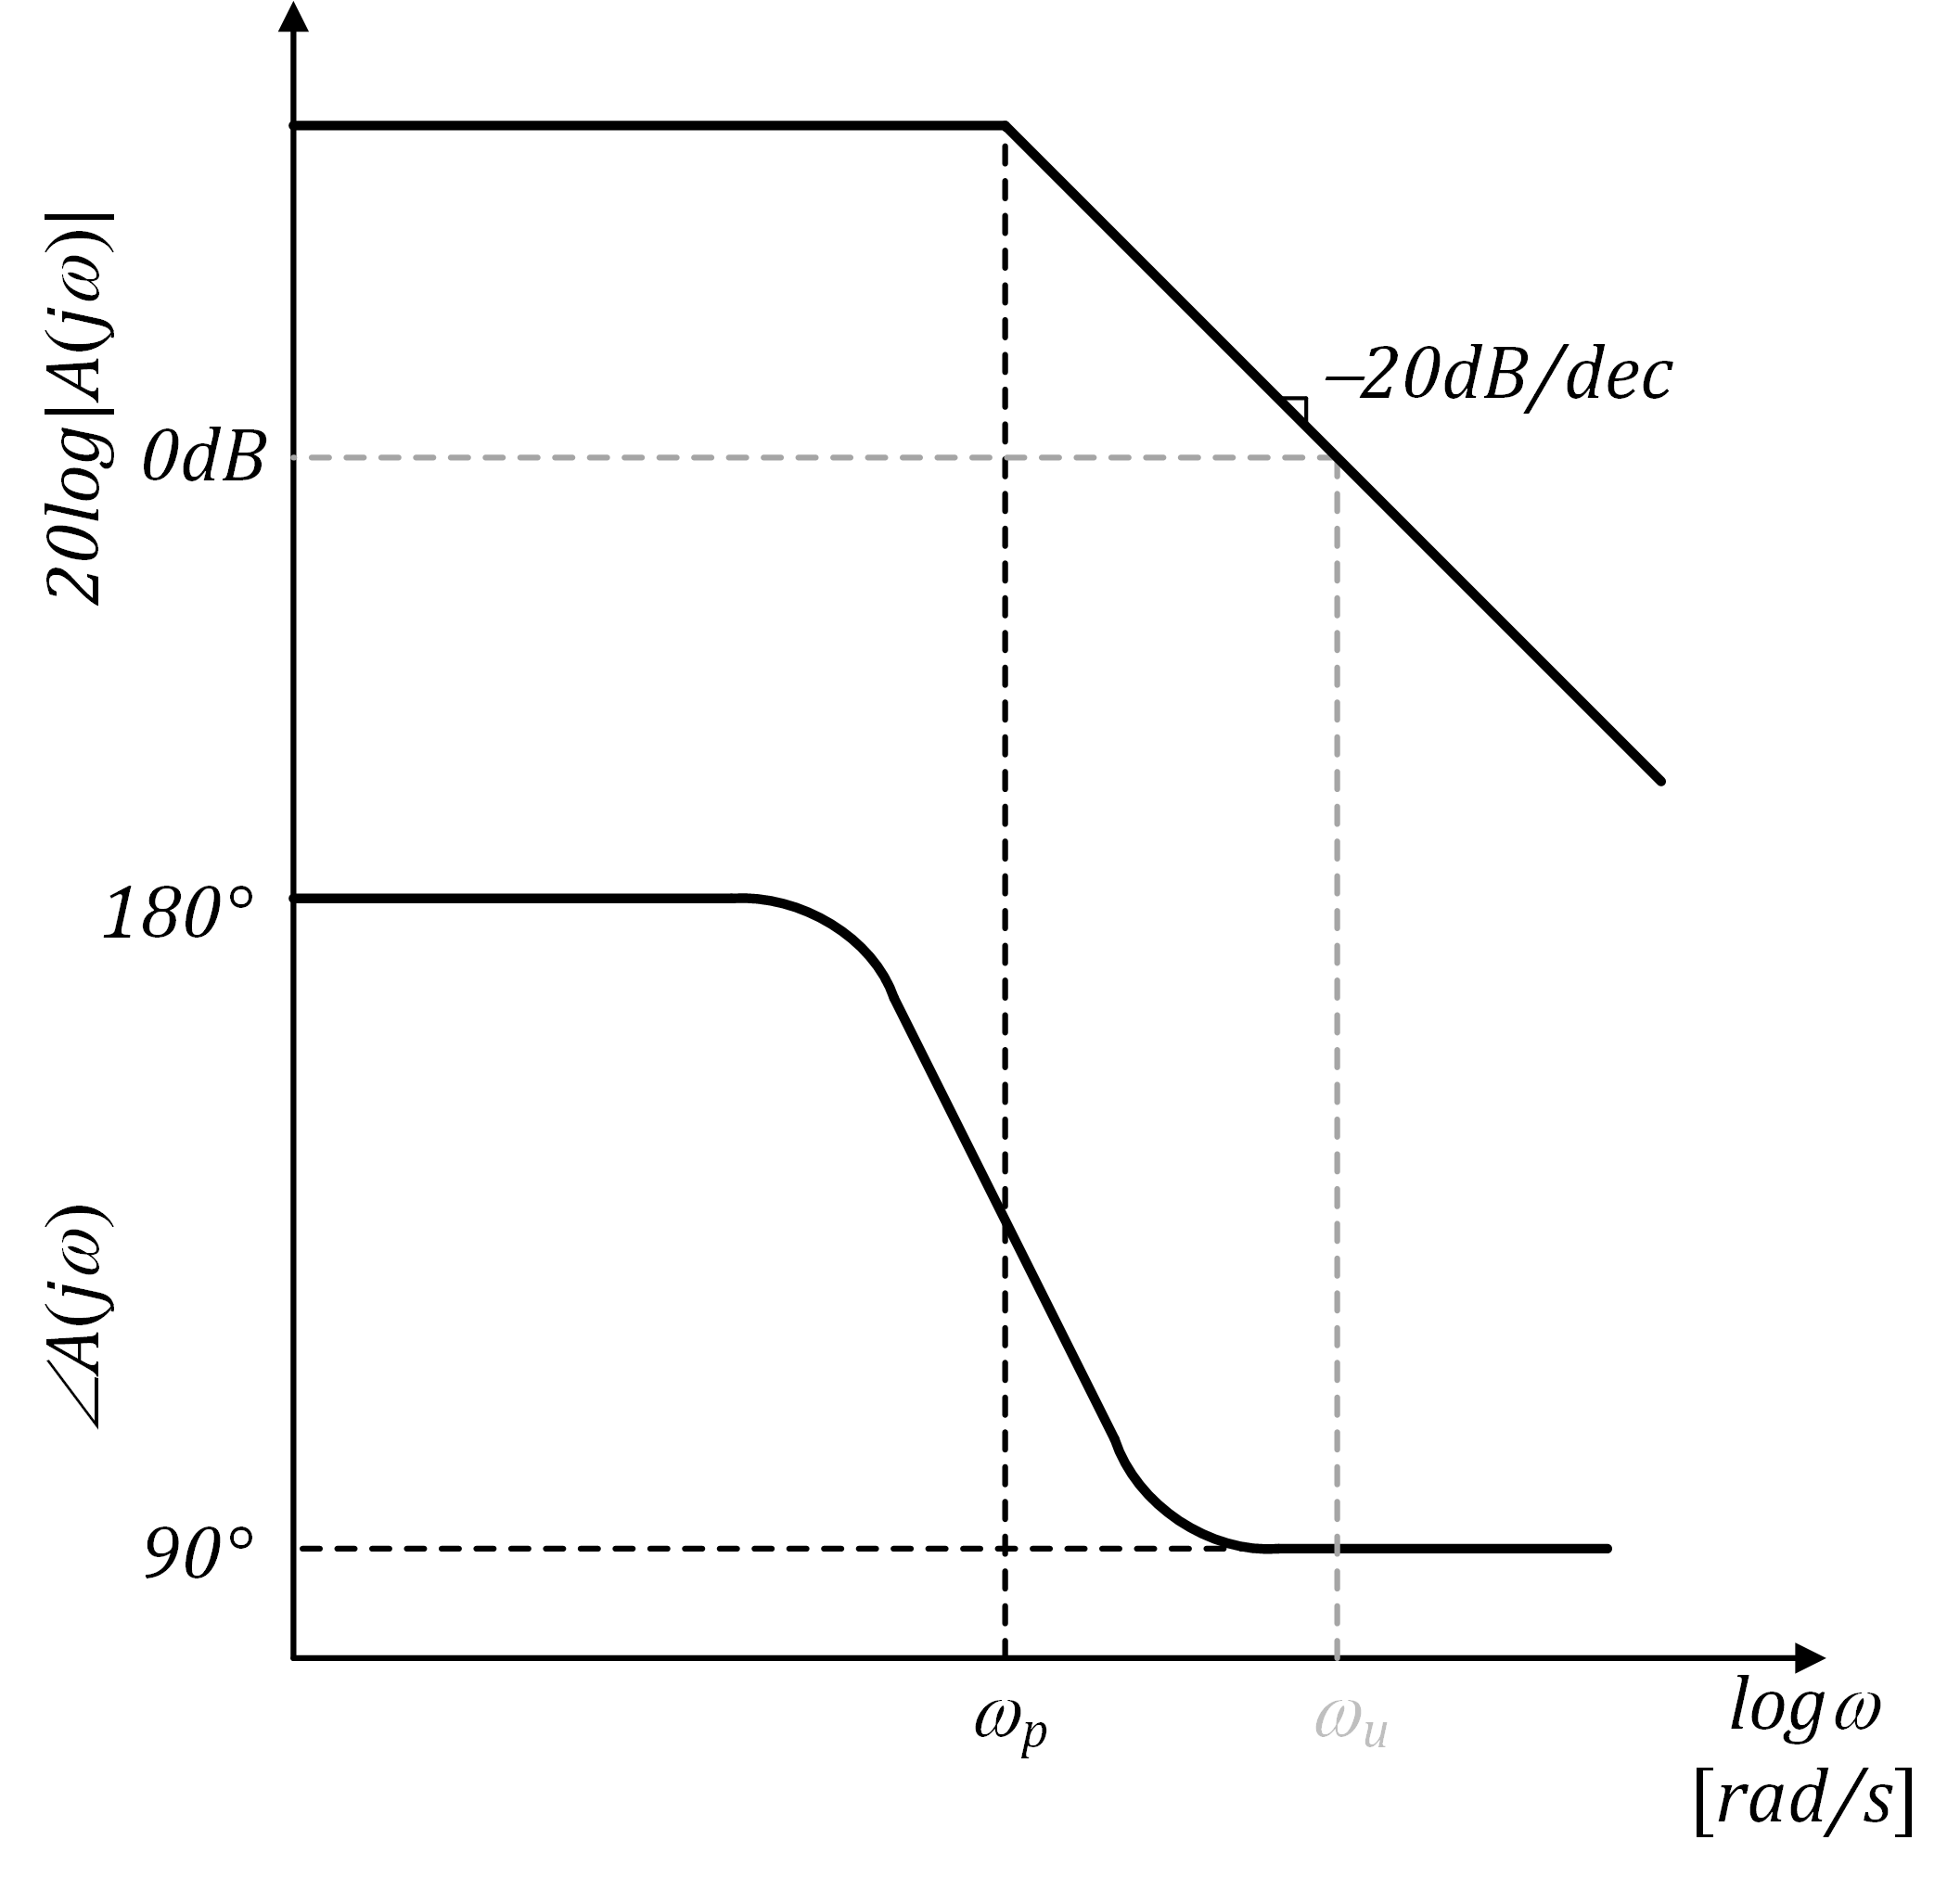
\includegraphics{phase_margin_first_order.png}
\caption{phase\_margin\_first\_order.png}
\end{figure}

    \begin{itemize}
\tightlist
\item
  Here, phase margin is defined as
\end{itemize}

\begin{equation}
PM = \angle A(j\omega_u) - 0^{\circ}
\end{equation}

\begin{itemize}
\tightlist
\item
  For a single-pole system, the phase margin is
\end{itemize}

\begin{equation}
PM = \angle A(j\omega_u) = 180^{\circ} - \tan^{-1}\dfrac{\omega_u}{\omega_{p1}}
\end{equation}

\begin{itemize}
\tightlist
\item
  This has a minimum value of
\end{itemize}

\begin{equation}
PM \geq 180^{\circ} - 90^{\circ} = 90^{\circ}
\end{equation}

\begin{itemize}
\tightlist
\item
  This guarantees stability and a ``well behaved'' step response
\end{itemize}

    \hypertarget{phase-margin-of-a-two-pole-system}{%
\subsection{Phase margin of a two-pole
system}\label{phase-margin-of-a-two-pole-system}}

    \begin{figure}
\centering
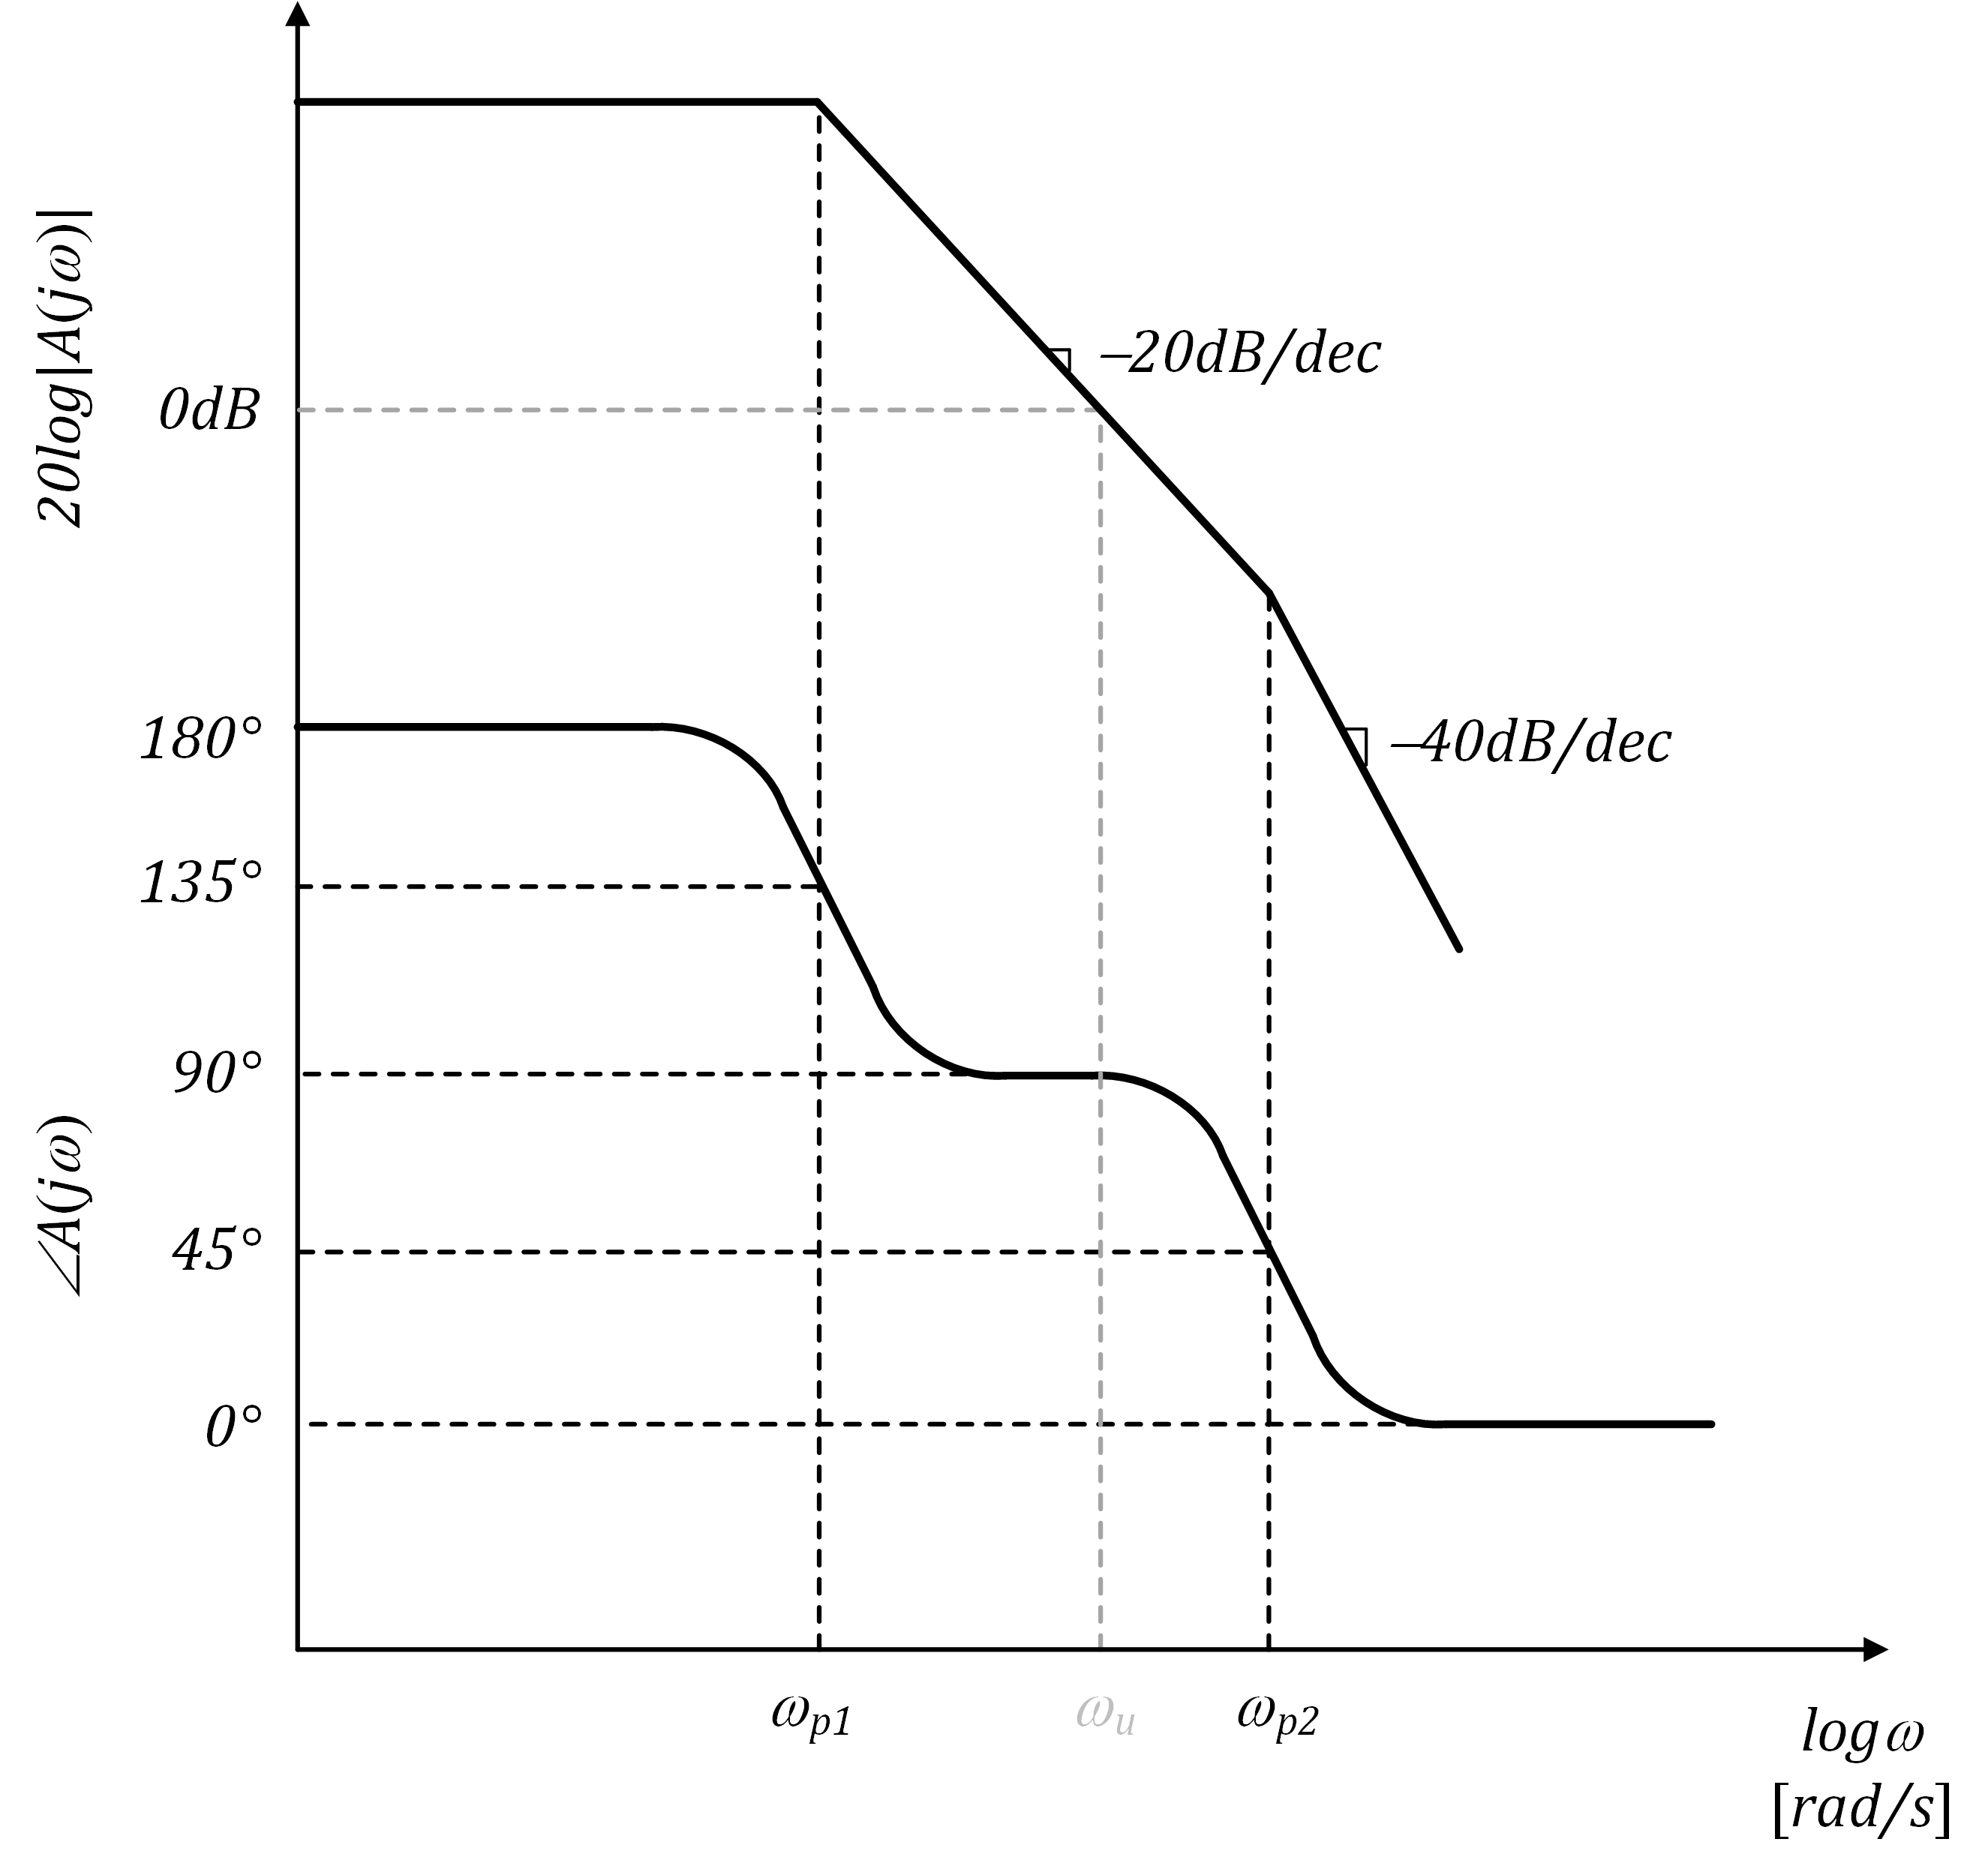
\includegraphics{phase_margin_second_order.png}
\caption{phase\_margin\_second\_order.png}
\end{figure}

    \begin{itemize}
\tightlist
\item
  For stability (i.e.~no oscillation), we need
\end{itemize}

\begin{equation}
\angle A(j\omega_u) > 0^{\circ}
\end{equation}

\begin{itemize}
\tightlist
\item
  For a well-behaved response, we prefer to have
\end{itemize}

\begin{equation}
\angle A(j\omega_u) \geq 60^{\circ}
\end{equation}

\begin{equation}
PM = \angle A(j\omega_u) = 180^{\circ} - \tan^{-1}\dfrac{\omega_u}{\omega_{p1}} - \tan^{-1}\dfrac{\omega_u}{\omega_{p2}}
\end{equation}

\begin{itemize}
\tightlist
\item
  This places a requirement on \(\omega_{p2}\) of
\end{itemize}

\begin{equation}
\tan^{-1}\dfrac{\omega_u}{\omega_{p2}} \leq 30^{\circ}
\end{equation}

\begin{equation}
\boxed{\omega_{p2} \geq 1.73\omega_u}
\end{equation}

    \hypertarget{telescopic-cascode-amplifier}{%
\subsection{Telescopic cascode
amplifier}\label{telescopic-cascode-amplifier}}

    \begin{figure}
\centering
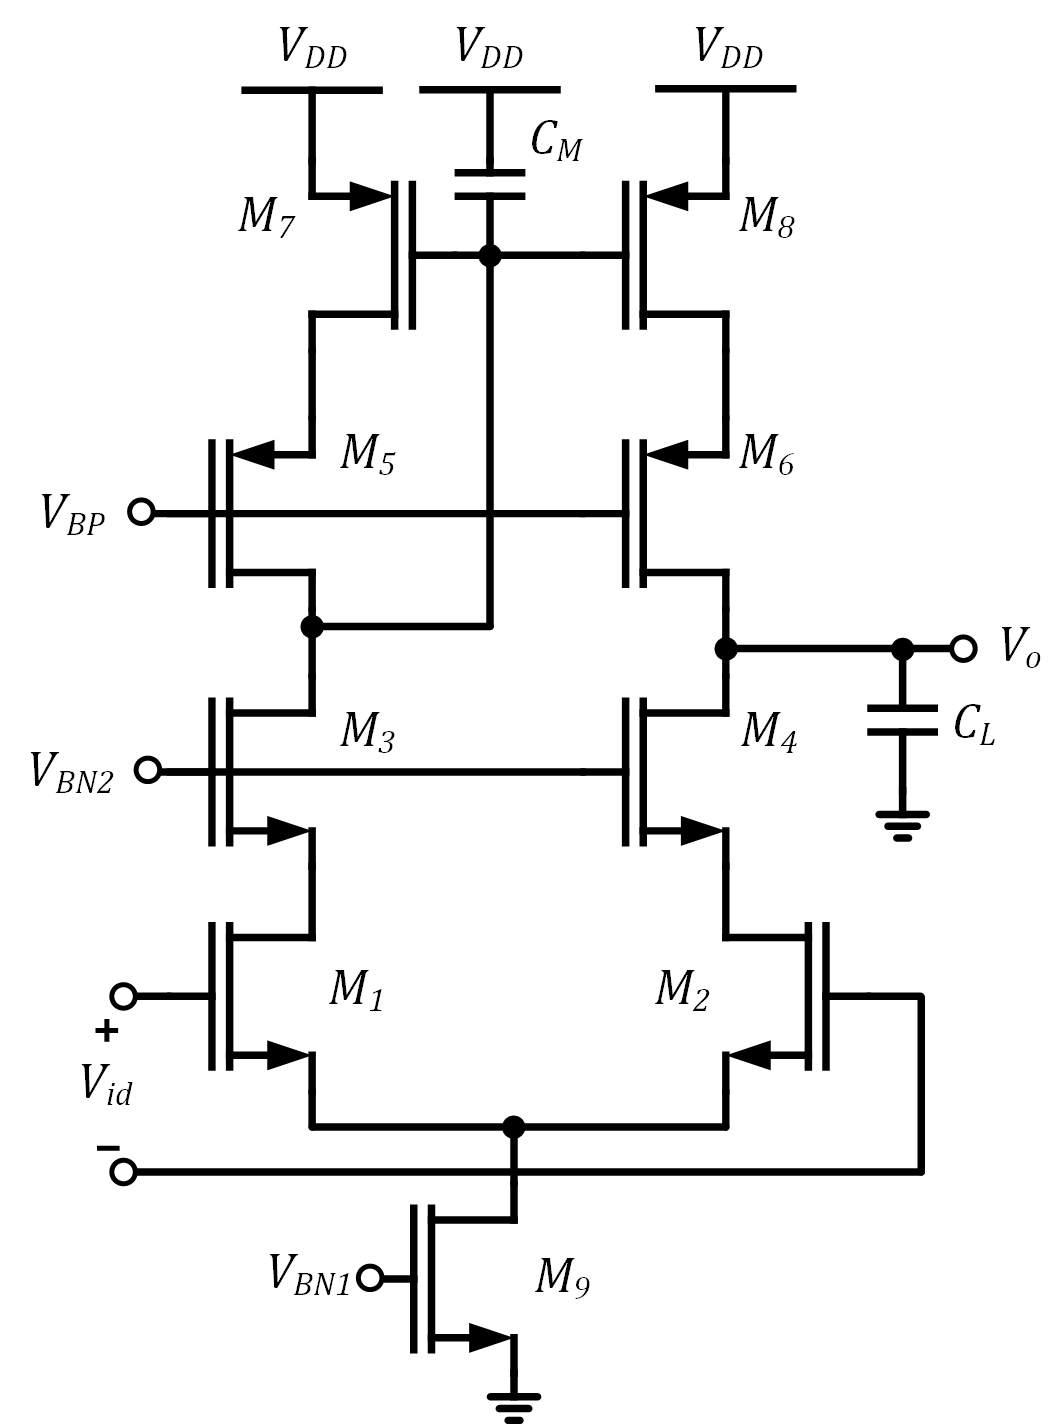
\includegraphics{telescopic_cascode_Cm.png}
\caption{telescopic\_cascode\_Cm.png}
\end{figure}

    \begin{itemize}
\item
  \(C_M\) represents parasitic capacitance at the gate node of \(M_7\),
  \(M_8\)
\item
  \(C_M\) may be large if \(V_{OV7,8}\) is small
\item
  \(M_7\) gate connection functions as a diode-connected MOS in the
  small-signal model
\item
  The \(3dB\) frequency can be found by ZVTC analysis, but assuming
  \(C_L >> C_M\), it can be approximated as the inverse of product of
  \(R_o\) and \(C_L\)
\end{itemize}

    \hypertarget{m7-diode-connection-small-signal-analysis}{%
\subsection{M7 diode connection (small signal
analysis)}\label{m7-diode-connection-small-signal-analysis}}

    \begin{figure}
\centering
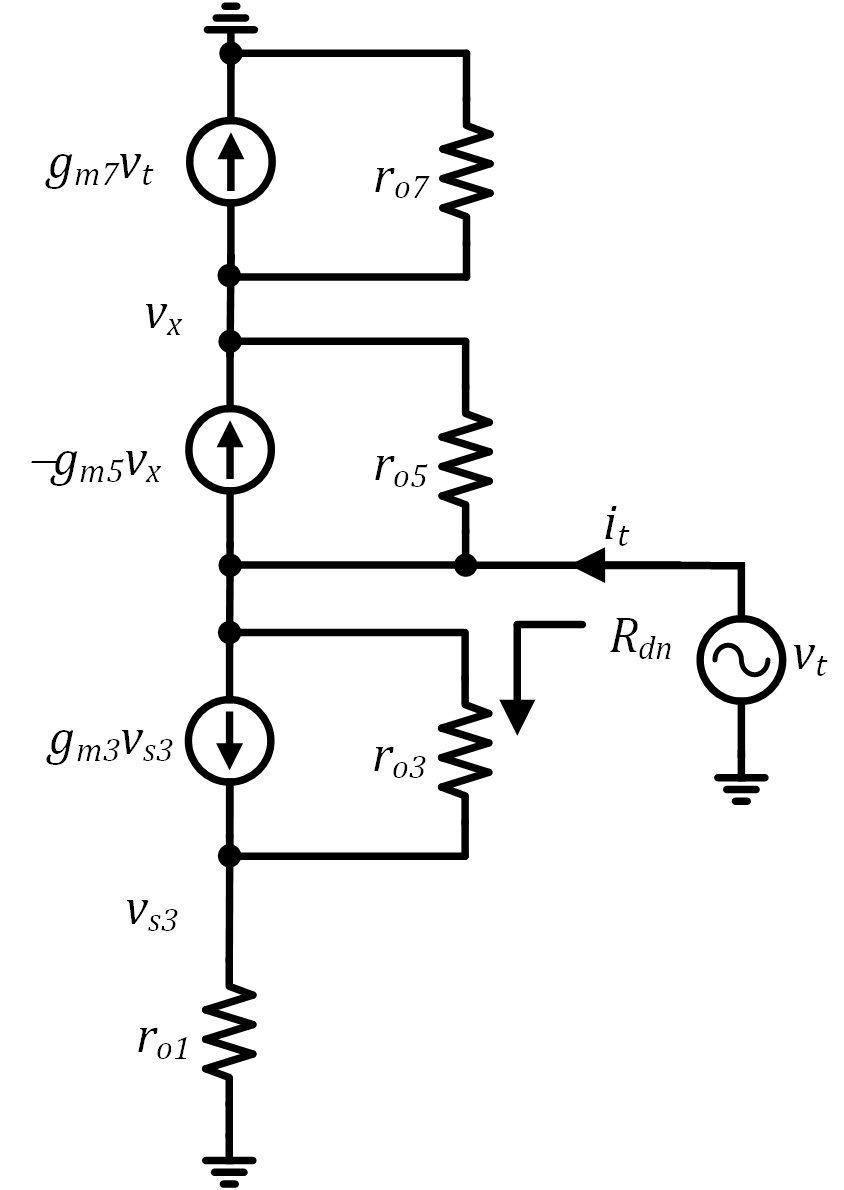
\includegraphics{mirror_pole_small_signal.png}
\caption{mirror\_pole\_small\_signal.png}
\end{figure}

    \begin{equation}
i_{up} = \dfrac{v_t - v_x}{r_{o5}} - g_{m5}v_x \:\:\:\:\:\:\: v_x = \dfrac{v_t - i_{up}r_{o5}}{g_{m5}r_{o5}+1}
\end{equation}

\begin{equation}
i_{up} = g_{m7}v_t+\dfrac{v_x}{r_{o7}} = g_{m7}v_t + \dfrac{v_t-i_{up}r_{o5}}{r_{o7}(g_{m5}r_{o5}+1)}
\end{equation}

\begin{equation}
i_{up}\left(1+\dfrac{r_{o5}}{r_{o7}(g_{m5}r_{o5}+1)}\right) = v_t\left(g_{m7}+\dfrac{1}{r_{o7}(g_{m5}r_{o5}+1)}\right)
\end{equation}

\begin{itemize}
\tightlist
\item
  The output resistance is thus
\end{itemize}

\begin{equation}
\boxed{R_{up} = \dfrac{v_t}{i_{up}}\approx \dfrac{1}{g_{m7}} \approx \dfrac{v_t}{i_t}}
\end{equation}

    \hypertarget{telescopic-amplifier-frequency-response}{%
\subsection{Telescopic amplifier frequency
response}\label{telescopic-amplifier-frequency-response}}

    \begin{figure}
\centering
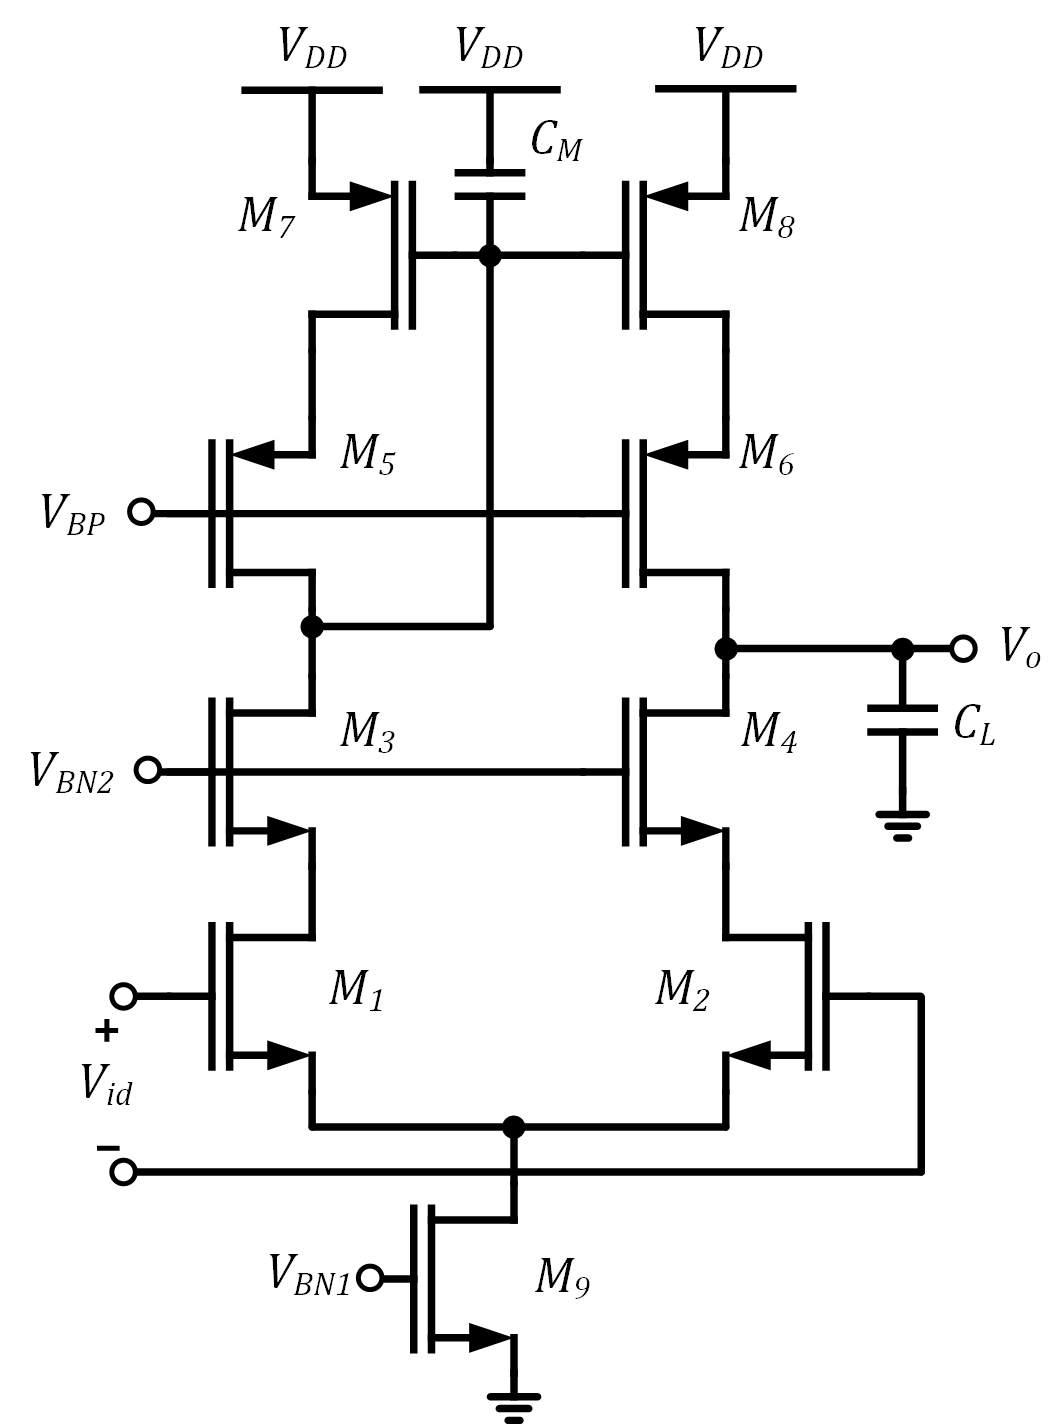
\includegraphics{telescopic_cascode_Cm.png}
\caption{telescopic\_cascode\_Cm.png}
\end{figure}

    \begin{itemize}
\tightlist
\item
  The dominant pole frequency is
\end{itemize}

\begin{equation}
\omega_{p1} \approx \dfrac{1}{g_{m6}r_{o6}r_{o8}||g_{m4}r_{o4}r_{o2} \cdot C_L}
\end{equation}

\begin{itemize}
\tightlist
\item
  The non-dominant pole is given by
\end{itemize}

\begin{equation}
\omega_{p2} \approx \dfrac{g_{m7}}{C_M}
\end{equation}

\begin{itemize}
\tightlist
\item
  Assuming \(\omega_{p2} >> \omega{p1}\), the gain-bandwidth is
\end{itemize}

\begin{equation}
\omega_u \approx \dfrac{g_{m1,2}}{C_L}
\end{equation}

\begin{itemize}
\tightlist
\item
  The phase is
\end{itemize}

\begin{equation}
\angle A(j\omega) = 180^{\circ} - \tan^{-1}\dfrac{\omega}{\omega_{p1}} - \tan^{-1}\dfrac{\omega}{\omega_{p2}}
\end{equation}

    \hypertarget{telescopic-amplifier-phase-margin}{%
\subsection{Telescopic amplifier phase
margin}\label{telescopic-amplifier-phase-margin}}

    \begin{figure}
\centering
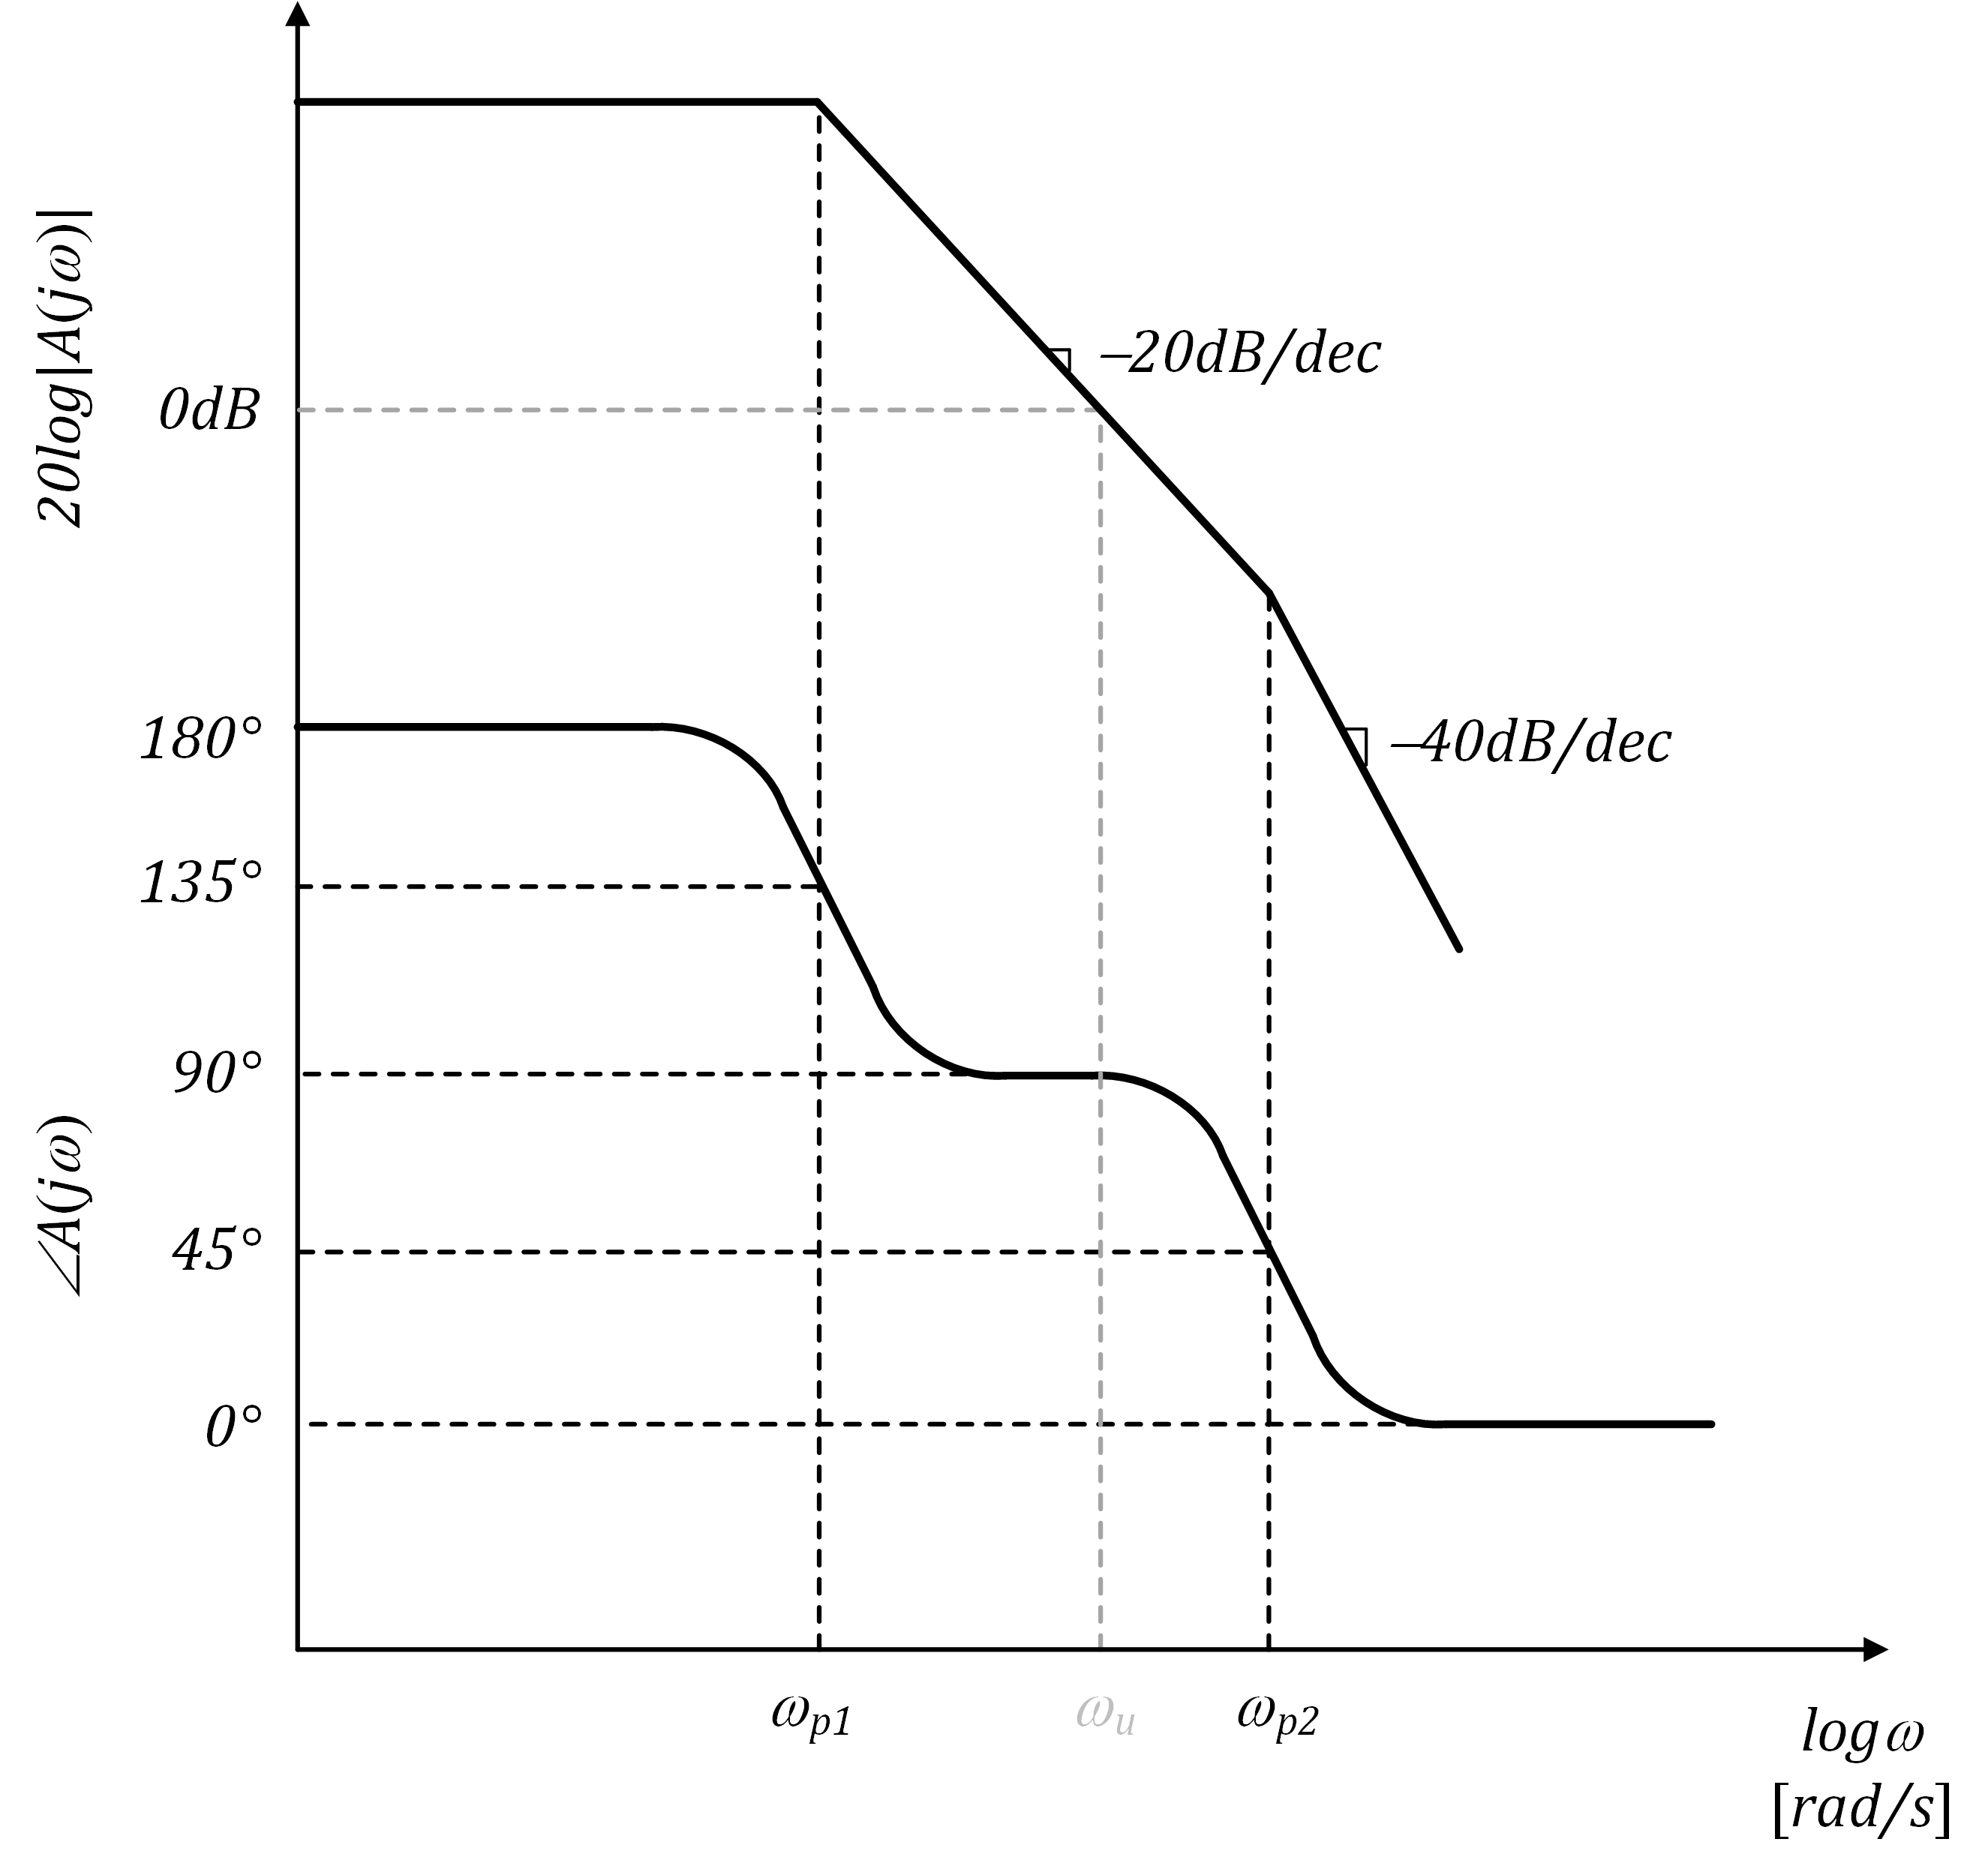
\includegraphics{phase_margin_second_order.png}
\caption{phase\_margin\_second\_order.png}
\end{figure}

    \begin{itemize}
\tightlist
\item
  For a well-behaved response we need
\end{itemize}

\begin{equation}
A(j\omega_u) \geq 60^{\circ}
\end{equation}

\begin{itemize}
\tightlist
\item
  Assuming a two-pole amplifier, this requires
\end{itemize}

\begin{equation}
\dfrac{g_{m7}}{C_M} \geq 1.73 \dfrac{g_{m1,2}}{C_L}
\end{equation}

\begin{itemize}
\tightlist
\item
  Using the long-channel model, the non-dominant pole can be expressed
  as
\end{itemize}

\begin{equation}
\dfrac{g_{m7}}{C_M} \approx \dfrac{\mu_p C_{ox}\frac{W}{L}V_{OV7,8}}{2\cdot\dfrac{2}{3}WLC_{ox}} = \dfrac{\mu_p V_{OV7,8}}{\dfrac{4}{3}L^2}
\end{equation}

    \hypertarget{frequency-response-of-a-2-stage-amplifier}{%
\subsection{Frequency response of a 2-stage
amplifier}\label{frequency-response-of-a-2-stage-amplifier}}

    \begin{figure}
\centering
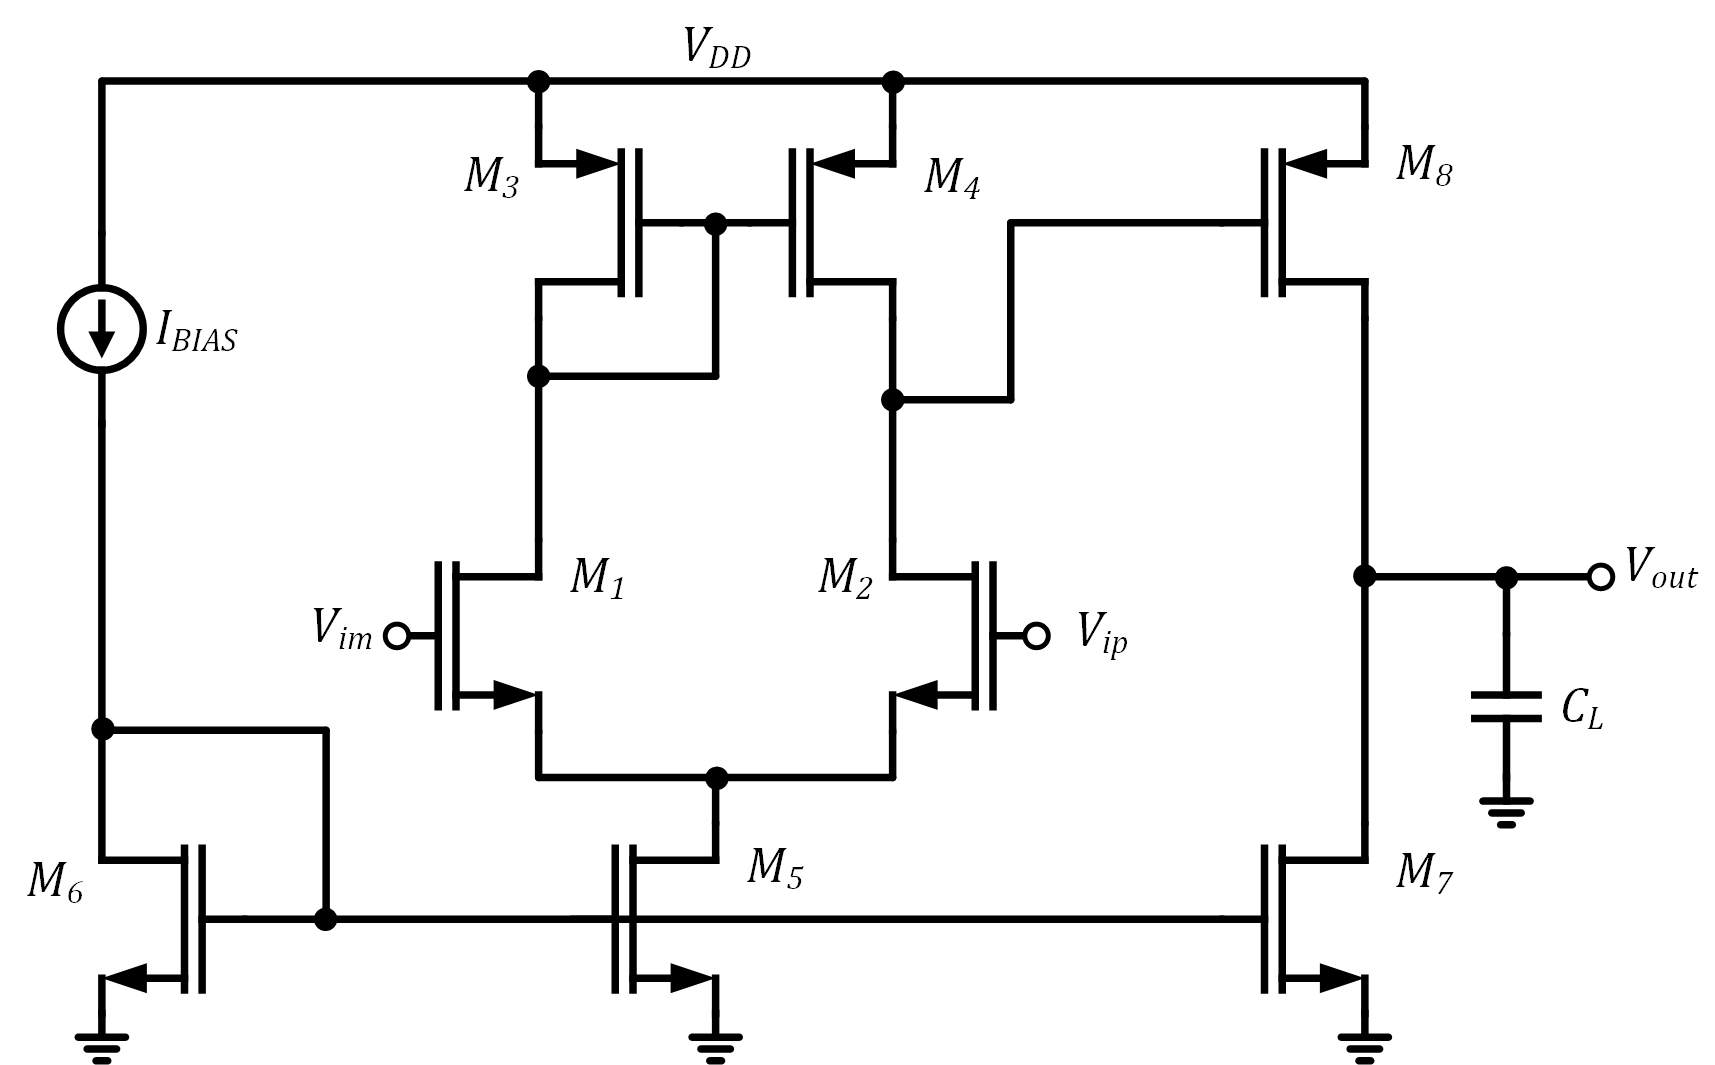
\includegraphics{2stage_OTA.png}
\caption{2stage\_OTA.png}
\end{figure}

    \begin{itemize}
\item
  A 2-stage amplifier can be analyzed in the same manner as a
  common-source amplifier
\item
  Here we primarily focus on the second stage, due to the high output
  impedance of the first stage (\(R_{o1} = r_{o2}||r_{o4}\)) and the
  Miller effect of \(M_8\)
\item
  The DC gain of the amplifier is given by the product of the gains of
  the individual stages:
\end{itemize}

\begin{align}
A_0 &= G_{m1}R_{o1}G_{m2}R_{o2}\\
&= g_{m1}r_{o2}||r_{o4}\cdot g_{m8}r_{o8}||r_{o7}
\end{align}

\begin{itemize}
\tightlist
\item
  Let's take a look at the frequency response\ldots{}
\end{itemize}

    \begin{itemize}
\tightlist
\item
  Assuming the mirror pole is well above the unity-gain bandwidth of the
  amplifier, the 2-stage CMOS OTA can be analyzed as a common-source
  amplifier with \(R_{o1} = r_{o2}||r_{o4}\) as the output impedance of
  the driving stage
\item
  In this case, the transfer function is given as
\end{itemize}

\begin{align}
A_v(s) &= g_{m1}R_{o1}\dfrac{(sC_{GD} - g_{m8})R_{o2}}{R_{o1} R_{o2}\xi s^2 + [R_{o1}(1+g_{m8}R_{o2})C_{GD} + R_{o1} C_{GS}+R_{o2}(C_{GD} + C_L)]s+1} \\
\end{align}

\begin{itemize}
\tightlist
\item
  If we allow \(R_{o2} \rightarrow \infty\) (this places the dominant
  pole at the origin), this becomes
\end{itemize}

\begin{align}
\lim_{R_{o2} \rightarrow \infty}{A_v(s)} &\approx g_{m1}R_{o1}\dfrac{(sC_{GD} - g_{m8})}{s[R_{o1}(C_{GS}C_{GD}+C_{GS}C_L+C_{GD}C_L)s + g_{m8}R_{o1}C_{GD} + (C_{GD} + C_L)]}\\
\end{align}

\begin{itemize}
\tightlist
\item
  The assumption that \(R_{o2} \rightarrow \infty\) is equivalent to the
  second stage being a ``perfect integrator'' (i.e.~infinite gain).
\end{itemize}

    \begin{itemize}
\tightlist
\item
  We can solve for the non-dominant pole by setting the denominator
  equal to zero and solving for \(s\). This gives
\end{itemize}

\begin{equation}
\omega_{p2} \approx \dfrac{(g_{m8}R_{o1}+1)C_{GD}+C_L}{R_{o1}(C_{GS}C_{GD}+C_{GS}C_L+C_{GD}C_L)
}\end{equation}

\begin{itemize}
\tightlist
\item
  This can be further approximated by assuming
  \(g_{m}R_{o1}C_{GD} >> C_L\)
\end{itemize}

\begin{equation}
\omega_{p2} \approx \dfrac{g_{m8}R_{o1}C_{GD}}{R_{o1}(C_{GD}(C_{GS}+C_L)+C_{GS}C_L)
}\end{equation}

\begin{itemize}
\tightlist
\item
  We have previously shown the dominant pole of the transfer function to
  be well-approximated as
\end{itemize}

\begin{equation}
\omega_{p1} \approx \dfrac{1}{R_{o1}(1+g_{m8} R_{o2})C_{GD}}
\end{equation}

    \hypertarget{pole-splitting}{%
\subsection{Pole splitting}\label{pole-splitting}}

    \begin{itemize}
\tightlist
\item
  With the two poles of the transfer function given by
\end{itemize}

\begin{equation}
\omega_{p1} \approx \dfrac{1}{R_{o1}(1+g_{m8} R_{o2})C_{GD}} \:\:\:\:\:\:\:\:\: \omega_{p2} \approx \dfrac{g_{m8}C_{GD}}{C_{GD}(C_{GS}+C_L)+C_{GS}C_L}
\end{equation}

\begin{itemize}
\item
  We can make some qualitative observations about their behavior:

  \begin{itemize}
  \tightlist
  \item
    As \(C_{GD}\) increases, \(\omega_{p1}\) decreases, lowering
    bandwidth
  \item
    \(\omega_{p2}\) simultaneously increases as the \(C_{GD}\) term in
    the denominator becomes dominant
  \item
    \(\omega_{p2}\) is ultimately limited by
    \(g_{m8}/(C_{GS} + C_L) \approx g_{m8}/C_L\)
  \end{itemize}
\item
  This behavior is referred to as ``pole splitting,'' since
  \(\omega_{p1}\) and \(\omega_{p2}\) are moving in opposite directions
  as \(C_{GD}\) is increased
\end{itemize}

    \hypertarget{stage-amplifier-rhp-zero}{%
\subsection{2-stage amplifier RHP zero}\label{stage-amplifier-rhp-zero}}

    \begin{itemize}
\tightlist
\item
  The full transfer function is once again given by
\end{itemize}

\begin{align}
A_v(s) &= \dfrac{(sC_{GD} - g_{m8})R_{o2}}{R_{o1} R_{o2}\xi s^2 + [R_{o1}(1+g_{m8}R_{o2})C_{GD} + R_{o1} C_{GS}+R_{o2}(C_{GD} + C_L)]s+1} \\
\end{align}

\begin{itemize}
\tightlist
\item
  The expression in the numerator,
  \(N(j\omega) = (sC_{GD} - g_{m8})R_{o2}\) results in a zero in the
  right half of the complex plane
\end{itemize}

\begin{equation} 
\omega_z = \dfrac{g_{m8}}{C_{GD}}
\end{equation}

\begin{itemize}
\tightlist
\item
  A zero in the right-half plane increases phase lag as well as gain
  magnitude, which can be detrimental to stability
\end{itemize}

\begin{equation}
\angle N(j\omega) = \tan^{-1}\left(-\dfrac{\omega C_{GD}}{g_{m8}}\right)
\end{equation}

    \hypertarget{phase-margin}{%
\subsection{Phase margin}\label{phase-margin}}

    \begin{itemize}
\tightlist
\item
  If we assume dominant-pole behavior, we can approximate the unity-gain
  frequency as
\end{itemize}

\begin{equation}
\omega_u \approx g_{m1}R_{o1}g_{m8}R_{o2} \cdot \dfrac{1}{g_{m8}R_{o2}R_{o1}C_{GD}} = \dfrac{g_{m1}}{C_{GD}}
\end{equation}

\begin{itemize}
\tightlist
\item
  The phase margin can then be approximated as
\end{itemize}

\begin{align}
PM &\approx 90^{\circ} - \tan^{-1}\dfrac{\omega_u}{\omega_{p2}} - \tan^{-1}\dfrac{\omega_u}{\omega_{z}} \\
&= \boxed{90^{\circ} - \tan^{-1}\dfrac{g_{m1}C_L}{g_{m8}C_{GD}} - \tan^{-1}\dfrac{g_{m1}}{g_{m8}}}\\
\end{align}

\begin{itemize}
\tightlist
\item
  Note that if \(g_{m1}\) and \(g_{m8}\) are comparable, and if
  \(C_L \geq C_{GD}\), the phase margin will be zero, or even negative!
\end{itemize}

    \hypertarget{frequency-response}{%
\subsection{Frequency response}\label{frequency-response}}

    \begin{tcolorbox}[breakable, size=fbox, boxrule=1pt, pad at break*=1mm,colback=cellbackground, colframe=cellborder]
\prompt{In}{incolor}{5}{\boxspacing}
\begin{Verbatim}[commandchars=\\\{\}]
\PY{n}{gm1} \PY{o}{=} \PY{l+m+mf}{1e\PYZhy{}3}
\PY{n}{gm8} \PY{o}{=} \PY{l+m+mf}{1e\PYZhy{}3}
\PY{n}{ro} \PY{o}{=} \PY{l+m+mf}{100e3}
\PY{n}{R\PYZus{}o1} \PY{o}{=} \PY{n}{ro}\PY{o}{/}\PY{l+m+mi}{2} 
\PY{n}{R\PYZus{}o2} \PY{o}{=} \PY{n}{ro}\PY{o}{/}\PY{l+m+mi}{2}
\PY{n}{C\PYZus{}GD} \PY{o}{=} \PY{l+m+mf}{1e\PYZhy{}12}
\PY{n}{C\PYZus{}GS} \PY{o}{=} \PY{o}{.}\PY{l+m+mf}{2e\PYZhy{}12}
\PY{n}{C\PYZus{}L} \PY{o}{=} \PY{l+m+mf}{1e\PYZhy{}12}
\PY{n}{zeta} \PY{o}{=} \PY{n}{C\PYZus{}GS}\PY{o}{*}\PY{n}{C\PYZus{}GD} \PY{o}{+} \PY{n}{C\PYZus{}GS}\PY{o}{*}\PY{n}{C\PYZus{}L}\PY{o}{+}\PY{n}{C\PYZus{}GD}\PY{o}{*}\PY{n}{C\PYZus{}L}
\PY{n}{num} \PY{o}{=} \PY{p}{[}\PY{n}{C\PYZus{}GD}\PY{o}{*}\PY{n}{R\PYZus{}o2}\PY{o}{*}\PY{n}{gm1}\PY{o}{*}\PY{n}{R\PYZus{}o1}\PY{p}{,} \PY{o}{\PYZhy{}}\PY{n}{gm8}\PY{o}{*}\PY{n}{R\PYZus{}o2}\PY{o}{*}\PY{n}{gm1}\PY{o}{*}\PY{n}{R\PYZus{}o1}\PY{p}{]}
\PY{n}{den} \PY{o}{=} \PY{p}{[}\PY{n}{R\PYZus{}o1}\PY{o}{*}\PY{n}{R\PYZus{}o2}\PY{o}{*}\PY{n}{zeta}\PY{p}{,} \PY{n}{gm1}\PY{o}{*}\PY{n}{R\PYZus{}o1}\PY{o}{*}\PY{n}{R\PYZus{}o2}\PY{o}{*}\PY{n}{C\PYZus{}GD}\PY{o}{+}\PY{n}{R\PYZus{}o1}\PY{o}{*}\PY{n}{C\PYZus{}GS}\PY{o}{+}\PY{n}{R\PYZus{}o2}\PY{o}{*}\PY{p}{(}\PY{n}{C\PYZus{}GD}\PY{o}{+}\PY{n}{C\PYZus{}L}\PY{p}{)}\PY{p}{,} \PY{l+m+mi}{1}\PY{p}{]}
\PY{n}{tf\PYZus{}CS} \PY{o}{=} \PY{n}{signal}\PY{o}{.}\PY{n}{TransferFunction}\PY{p}{(}\PY{n}{num}\PY{p}{,}  \PY{n}{den}\PY{p}{)}
\PY{n}{w}\PY{p}{,} \PY{n}{mag}\PY{p}{,} \PY{n}{phase} \PY{o}{=} \PY{n}{tf\PYZus{}CS}\PY{o}{.}\PY{n}{bode}\PY{p}{(}\PY{p}{)}       
\PY{n}{f} \PY{o}{=} \PY{n}{w}\PY{o}{/}\PY{l+m+mi}{2}\PY{o}{/}\PY{n}{np}\PY{o}{.}\PY{n}{pi}  
\end{Verbatim}
\end{tcolorbox}

    \begin{tcolorbox}[breakable, size=fbox, boxrule=1pt, pad at break*=1mm,colback=cellbackground, colframe=cellborder]
\prompt{In}{incolor}{6}{\boxspacing}
\begin{Verbatim}[commandchars=\\\{\}]
\PY{n}{plot\PYZus{}logxy2}\PY{p}{(}\PY{n}{f}\PY{p}{,} \PY{n}{mag}\PY{p}{,} \PY{n}{f}\PY{p}{,} \PY{n}{phase}\PY{p}{,} \PY{l+s+s1}{\PYZsq{}}\PY{l+s+s1}{Frequency [Hz]}\PY{l+s+s1}{\PYZsq{}}\PY{p}{,} \PY{l+s+s1}{\PYZsq{}}\PY{l+s+s1}{Magnitude [dB]}\PY{l+s+s1}{\PYZsq{}}\PY{p}{,}
           \PY{l+s+s1}{\PYZsq{}}\PY{l+s+s1}{Frequency [Hz]}\PY{l+s+s1}{\PYZsq{}}\PY{p}{,} \PY{l+s+s1}{\PYZsq{}}\PY{l+s+s1}{Phase [deg]}\PY{l+s+s1}{\PYZsq{}}\PY{p}{)}
\end{Verbatim}
\end{tcolorbox}

    \begin{center}
    \adjustimage{max size={0.9\linewidth}{0.9\paperheight}}{2021_02_24_EE538_Lecture8_W2021_files/2021_02_24_EE538_Lecture8_W2021_80_0.png}
    \end{center}
    { \hspace*{\fill} \\}
    
    \hypertarget{summary}{%
\subsection{Summary}\label{summary}}

    \begin{itemize}
\tightlist
\item
  The frequency response of closed-loop amplifiers relies on
  characteristics of the open-loop response
\item
  Stability of negative-feedback systems requires a phase lag of less
  than \(180^{\circ}\) at the transit (unity-gain) frequency
\item
  Bode plots and root loci can be used to evaluate stability of
  closed-loop systems
\item
  To ensure ``well-behaved'' closed-loop responses, phase margin should
  be kept above \textasciitilde{}\(60^{\circ}\) (overdamped, no
  overshoot)
\item
  Mirror pole can degrade phase margin in single-ended OTAs
\item
  2-stage OTAs have multiple poles and a RHP zero
\item
  Next time, we'll look at compensation of 2-stage CMOS OTAs
\end{itemize}


    % Add a bibliography block to the postdoc
    
    
    
\end{document}
